\documentclass[twoside,11pt,openright]{report}

\usepackage[utf8]{inputenc}
\usepackage[american]{babel}
\usepackage{a4}
\usepackage{latexsym}
\usepackage[numbers]{natbib}
%\usepackage[square,semicolon,sort,longnamesfirst]{natbib}
\usepackage{amssymb}
\usepackage{amsmath}
\usepackage{epsfig}
\usepackage{graphicx}
\usepackage[T1]{fontenc}
\usepackage{lmodern}
\usepackage{color}
\usepackage{datetime}
\usepackage{epstopdf} 

\usepackage{tikz}
\newcommand*\circled[1]{\tikz[baseline=(char.base)]{
    \node[shape=circle,draw,inner sep=2pt] (char) {#1};}}
\usepackage{caption}
\usepackage{subcaption}
\usepackage{epigraph}
\setlength\epigraphwidth{8cm}
\setlength\epigraphrule{0pt}

\usepackage{etoolbox}

\makeatletter
\patchcmd{\epigraph}{\@epitext{#1}}{\itshape\@epitext{#1}}{}{}
\makeatother

\renewcommand*\ttdefault{txtt}

\newcommand{\todo}[1]{{\color[rgb]{.5,0,0}\textbf{$\blacktriangleright$#1$\blacktriangleleft$}}}

\newtheorem{innercustomlem}{Lemma}
\newenvironment{customlem}[1]
  {\renewcommand\theinnercustomlem{#1}\innercustomlem}
  {\endinnercustomlem}

\newtheorem{innercustomthm}{Theorem}
\newenvironment{customthm}[1]
  {\renewcommand\theinnercustomthm{#1}\innercustomthm}
  {\endinnercustomthm}



% see http://imf.au.dk/system/latex/bog/

\begin{document}

%%%%%%%%%%%%%%%%%%%%%%%%%%%%%%%%%%%%%%%%%%%%%%%%%%%%%%%%%%%%%%%%%%%%%%%
\pagestyle{empty} 
\pagenumbering{roman} 
\vspace*{\fill}\noindent{\rule{\linewidth}{1mm}\\[4ex]
{\Huge\sf Orthogonal Range Searching in 2D with Ball Inheritance}\\[2ex]
{\huge\sf Mads Ravn, 20071580}\\[2ex]
\noindent\rule{\linewidth}{1mm}\\[4ex]
\noindent{\Large\sf Master's Thesis, Computer Science\\[1ex] 
\monthname\ \the\year  \\[1ex] Advisor: Kasper Green Larsen\\[15ex]}\\[\fill]}

\epsfig{file=logo.eps}\clearpage

%%%%%%%%%%%%%%%%%%%%%%%%%%%%%%%%%%%%%%%%%%%%%%%%%%%%%%%%%%%%%%%%%%%%%%%

\pagestyle{plain}
\chapter*{Abstract}
\addcontentsline{toc}{chapter}{Abstract}

This thesis studies orthogonal range searching which is one of the most well-studied problems in computational geometry. We introduce the Ball Inheritance Search data structure. This data structure requires $\mathcal{O}(n)$ space and can return $k$ points with a query time of $\mathcal{O}(\lg n + k\cdot\lg^\epsilon n)$ for any fixed constant $\epsilon > 0$. We compare the Ball Inheritance Search data structure to the kd-tree. The kd-tree requires $\mathcal{O}(n)$ space and can return $k$ points with a query time of $\mathcal{O}(\sqrt{n} + k)$.\\

We compare the query time of the two data structures with queries of different shapes. We show that both data structure have both best-case and worst-case shapes for their queries, and given a search query of their best-case shape they perform better than their counterpart.\\

Finally we look at a small amount of results. A search query of the worst-case shape to the Ball Inheritance Search data structure does not perform that much worse than the best-case shape to the kd-tree, while a search query of the best-case shape the Ball Inheritance Search performs much better than a search query of the worst-case shape to the kd-tree. The difference between the best-case and worst-case shape is least on the Ball Inheritance Search data structure, and thus it has a more stable performance.



\chapter*{Acknowledgements}
\addcontentsline{toc}{chapter}{Acknowledgments}

First and foremost, I would like to thank my thesis advisor, Kasper Green Larsen. He shared his idea for the thesis with me, and he has been extremely helpful and engaged in the process of my writing. It has been a great experience to work with Kasper.
I would also like to thank Eva Frederiksen for creating the figures in chapters $1$, $2$ and $3$. It obviously helps a lot when the figures make sense. Johan Abildskov was kind enough to read an early draft of my thesis and give me some very good feedback and ideas.\\

Some of the figures in this thesis are inspired by the figures in Computational Geometry: Algorithms and Applications\cite{compgeo}.

\vspace{2ex}
\begin{flushright}
  \emph{Mads Ravn,}\\
  \emph{Aarhus, \today.}
\end{flushright}

\tableofcontents
\pagenumbering{arabic}
\setcounter{secnumdepth}{2}

%%%%%%%%%%%%%%%%%%%%%%%%%%%%%%%%%%%%%%%%%%%%%%%%%%%%%%%%%%%%%%%%%%%%%%%


\chapter{Introduction}
\label{ch:intro}

\todo{Describe primary work}
In this thesis we are going to explore data structure we believe to be faster at orthogonal range search than a kd-tree. We are going to introduce the a range reporting data structure by \citet{chanetal}. A simplified version of their data structure will be made and implemented. We wish to show that this simplified version is able to compete with a kd-tree. \\

\noindent \textbf{Orthogonal Range Searching.} \emph{Orthogonal range searcing} is one of the most fundamental and well-studied problems in computational geometry. Even with extensive research over three decades a lot of questions remain. In this thesis we will focus on $2D$ orthogonal range searching: Given $n$ points from $\mathbb{R}^2$ we want to insert them into a data structure which will be able to efficiently report which $k$ points lie within a given query range $\mathbb{Q} \subseteq \mathbb{R}^2$. This query can be defined as two corners of a rectangle, the lower left corner and the upper right corner, seeing as the query range is orthogonal to the axes. \\

\noindent \textbf{RAM, I/O, pointer models} \todo{Skriv om Word RAM Model sammenlignet med de andre typer her. Når vi pakker bits ned i et word kan vi stadig tilgå det hele da access er constant time og operations er constant time}\\

\noindent \textbf{Rank Space Reduction.} Given $n$ points from a universe $U$, the rank of a given point in a sorted list is defined as the amount of points which preceed it in the list. Given two points $a,b \in U: a < b$ \emph{iff} $rank(a) < rank(b)$. Expanding this concept to 2 dimensions we have a set $P$ of $n$ points on a $U \times U$ grid. We compute for the \emph{x-rank} $r_x$ for each point in $P$ by finding the rank of the x-coordinate amongst all the x-coordinates in $P$. The \emph{y-rank} $r_y$ finds the rank of y-coordinate amongst all of the y-coordinates in $P$. Using \emph{rank space reduction} on $P$ a new set $P^*$ is constructed where $(x,y) \in P$ is replaced by $(r_x(x), r_y(y) \in P^*$. Given a range query $q = [x_1, x_2] \times [y_1, y_2]$, a point $(x,y) \in P$ is found within $q$ \emph{iff} $(r_x(x), r_y(y))$ is found within $q^* = [r_x(x_1), r_x(x_2)] \times [r_y(y_1), r_y(y_2)]$. \todo{Noget med at deres ordered property remains intact.} Computing the set $P^*$ from $P$ using rank space reduction, $P^*$ is said to be in rank space. While the $n$ points could be represented by $\lg U$ bits in $P$, they can now be represented by $\lg n$ bits in $P^*$ with $\lg n \ll \lg U$ when $n \ll U$ which saves memory. \todo{We have essentially created a mapping between \dots } \\

%\noindent \textbf{Ball Inheritance Problem.} Given a perfect binary tree with $n$ leaves, we want to distribute $n$ labelled balls which appear in an ordered list at the root to the leaves in $\lg n$ steps. \todo{Rephrase}. The list of balls at a given node will inherited by its children with each child receiving the same amount of balls. Each level of the tree contains the same amount of balls. Eventually each ball reaches a leaf of the tree and each leaf will contain exactly one ball. The identity of a given ball is a node and the index of the ball in that nodes list. The true identity, the information the ball contains, only lies in the leaf. The \emph{ball-inheritance problem} is to track a ball from a given node to a leaf and report the identity of the leaf. \\

\noindent \textbf{Ball Inheritance.} Given a perfect binary tree with $n$ leaves and $n$ labelled balls at the root, we wish to distribute the balls from the root to the leaves. The balls at the root are contained in an ordered list and for each ball in a nodes list one of its children is picked to inherit the ball such that both children recieve the same amount of balls. The level of a node is defined to be the height of the node from the bottom. The root has the highest level, while each node is one level smaller than its parent. The leaves are at level $0$. Each level of the tree contains the same amount of balls, and at level $i$ each node contains $2^i$ balls. Eventually each ball reaches a leaf of the tree and each leaf will contain exactly one ball. A ball can be identified by a node and the index of the ball in that node's list. Given the identity of a ball at any level, it is possible to follow this identity to its actual coordinates. The goal is to track a balls inheritance from a given node to a leaf and report the identity of the leaf. We call the identity of the leaf, where the actual coordinates reside, the \emph{true identity} of a ball. When refering to ball inheritance, the words \emph{ball} or \emph{point} can be used interchangebly. \\


\noindent \textbf{Outline.} Has yet to be written. \\

\noindent \textbf{Notation.} The set of integers $\{i, i+1, \dots, j-1, j\}$ is denoted by $[i,j]$. When no base is explicitely given logarithm will have base $2$. $\epsilon$ is an arbitrary small constant greater than $0$. Given an array $A$, $A[i]$ denotes the entry with index $i$ in $A$ and $A[i,j]$ denotes the subarray containing the entries from $i$ to $j$ in $A$. $A[1..n]$ denotes an array $A$ of size $n$ with entries $1$ to $n$. Throughout the thesis the successor of $x$ in a set will be meant as the first number which is greater or equal to $x$ in that set - the same applies for predecessor of $x$. The work will be done under the assumption that no two points will  have the same x-coordinate and no two points will have the same y-coordinate. This is a unrealistic assumption in practice, but it can easily be remedied by having the points lie in a \emph{composite-number space} since we only need a total ordering of our points.




%%%%%%%%%%%%%%%%%%%%%%%%%%%%%%%%%%%%%%%%%%%%%%%%%%%%%%%%%%%%%%%%%%%%%%%
\part{Theory}

\chapter{Related Work}
\label{ch:relatedwork}

In this chapter the original work of \citet{chanetal} is presented followed by a simplification of their idea. This simplification serves two purposes: It will be easier to implement which will present a much cleaner code to read and it will be easier to execute since it has much less things to compute and look up. The theory behind a $kD$-tree will also be explained as it is the de facto standard of orthogonal range queries today and will be used to compare the practical results of the simplified model.

This simplified range searching is still theoritically faster than the kd-tree which is the standard range search used today. 

\section{kd-trees}

The current standard of range reporting is kd-trees. This technique will be used as a reference point when evaluting the results of the primary work in this thesis. With linear space it is optimal for range reporting on the RAM.

A kd-tree is constructed recursively: Given $n$ points, the median of the points with respect to x are found. All points which has an x-coordinate larger than the median goes to the right child, while points which has an x-coordinate smaller than the median, and the median point, goes to the left child. At the next level the points will be divived in a similar fashion, this time using the y-median and the y-coordinates instead. When dividing $n$ points, the median will be chosen as the $\lceil n/2 \rceil$-th smallest number \cite{compgeo}.
Switching back and forth between focussing on x or y is done at each level of the tree and this will be continued until a binary tree has been constructed with $n$ leaves.

The tree with $n$ points can be represented as flat array with $n$ entries. The $\lceil n/2 \rceil$-th element in the array is the root of the tree. And so forth.
 With this in mind, the entire tree can represented using a flat array with $n$ elements. 




\section{Original Range Searching}
\label{sect:original}
Utilizing the \emph{ball inheritance} concept \citeauthor{chanetal} propose a better solution for ranged search queries. With the same space complexity as the $kD$-tree, but lower query time. Theorem $2.1$ states that \emph{for any $2 \leq B \leq \lg^\epsilon n$, we can can solve $2$-d orthogonal range reporting in rank space with $\mathcal{O}(n \lg_B \lg n)$ space and $(1+k)\mathcal{O}(B \lg \lg n)$ query time.}

\subsection{Solving the ball-inheritance problem} 
\label{ssection:solving-ball}

Consider a perfect binary tree with $n$ leaves. At each level we use a bit vector $A[1..n]$ to indicate which of its children a ball is inherited by: If $A[i]$ is $0$ means that the ball with identity $i$ in that node was inherited by its left child and $1$ means that it was inherited by its right child. Given a node and an identity of a ball we can know calculate the balls identity in the node it is inherited by. The node can answer the query $rank(k) = \Sigma_{i \leq k} A[i]$. If a ball is inherited by the right child node its new identity at that node is $rank(i)$ because that is how many $1$s that preceeds it in the current node. If a ball is inherited by the left child node the new identity is then $i-rank(i)$. With this information it is possible to traverse down the tree following a ball from any given node to a leaf. There are n balls per level which is represented by a bit vector of size $n$ per level, so even though conceptually this bit vector is divided out amongst the nodes of that level, we can interchangebly think of a bit vector per level or a bit vector per node.\todo{Rephrase and replace} Each level in the tree uses $\mathcal{O}(n)$ bits to store the bit vectors. This adds up to $\mathcal{O}(n \lg n)$ bits, or $\mathcal{O}(n)$ words. This trivial solution to the ball-inheritance problem uses $\mathcal{O}(\lg n)$ query time. \\


A bit vector is an array with entries from the alphabet $\Sigma = {0,1}$, where each entry is used to indicate whether a left or right child has been chosen for ball inheritance. By expanding the alphabet we can point to the childrens children, $\Sigma = \{0,1,2,3\}$, the childrens childrens children, $\Sigma = \{0,1,2,3,4,5,6,7\}$, and so forth. Expanding the alphabet will use $\mathcal{O}(n \lg \Sigma)$ bits per level. Storing a pointer from level $i$ to level $i+\Delta$ increases the storage space by $\Delta$ bits per ball, but also enables the ball to be inherited by $2^\Delta$ descendants. By expanding the alphabet the query time can be lowered since it is possible to take bigger steps down the tree. 

Using this concept, we pick $B$ such that $2 \leq B \leq m$. All levels that are a multiple of $B^i$ expand their alphabet such that the balls can reach $B^i$ levels down. If the level does not exist, the ball points to its leaf. We need at most visit $B$ levels that are multiple of $B^i$ before reaching a level that is multiple of $B^{i+1}$, making it possible to jump down the tree with bigger and bigger steps.

Storing the expanded alphabets at each level that is multiple of $B^i$ costs $B^i$ bits per ball. The total cost is then $\Sigma_i \frac{\lg n}{B^i} * \mathcal{O}(B^i) = \mathcal{O}(\lg n * \lg_B \lg n)$ bits per ball (at all levels). With $n$ balls, this is $\mathcal{O}(n \lg_B \lg n)$ words of space with query time of $\mathcal{O}(B \lg_B \lg n)$. \todo{Spørg Kasper med matematikken bag dette - især om ``at all levels'' er rigtig og hvordan $\Sigma$ forvandles til $\lg_B \lg n$}


\subsection{Solving range reporting}
With a solution to the ball-inheritance problem, \citet{chanetal} proposes \textbf{Lemma 2.4} \emph{if the ball inheritance problem can be solved with space $S$ and query time $\tau$, $2$-d range reporting can be solved with space $\mathcal{O}(S+n)$ and query time $\mathcal{O}(\lg \lg n + (1+k) \tau)$.}

Consider a perfect binary tree with $n$ leaves. The root contains $n$ points in $2$-d rank space. These $n$ balls are sorted by their y-rank and will keep this order all the way down the tree. When distributing the balls for inheritance, a node will give both its children half of its balls. The lower half sorted by the x-rank to its left child and the upper half by x-rank to its right child. The actual coordinates of the balls are only stored at the leaves and we know that x-coordinates of the balls in the leaves are sorted from left to right - smallest to highest. Since we only store the actual coordinate points once this data structure uses linear space.

Having distributed the $n$ points from the root to the leaves, we require additional data structures in order to answer the range queries. We will use a succint data structure for the \emph{range minimum query}. Consider an array $A$ with $n$ comparable keys, the goal is to find the index of the minimum key in the subarray $A[j,i]$. \todo{Describe either the cartesian tree or reference 29}. For each node in the tree that is a right child we add a range minimum query structure. The indices are the y-rank and the keys are the x-rank that the given node contains. A range maximum query structure is added to the all the nodes which are left children. Each data structure uses an amount of bits linear of the size of the nodes ball list, making it $\mathcal{O}(n)$ bits per level of the tree and $\mathcal{O}(n \lg n)$ bits in all - i.e. $\mathcal{O}(n)$ words of space. \todo{What is the query time of this structure?}\\

There is still the matter of adding predecessor (and successor) search for the y-rank.
For this purpose a succint data structure is added to some levels of the tree. Given a sorted array $A[1..n]$ of $\omega$-bit integers, predecessor search queries in $\mathcal{O}(\lg \omega)$ time is supported using $\mathcal{O}(n \lg \omega)$ space which has oracle access to the entries in the array. \todo{reference}. The points in rank space of $\mathcal{O}(\lg n)$ bits will use $\mathcal{O}(n \lg \lg n)$ bits ($\omega = \lg n$) per level and $\mathcal{O}(n \lg n \lg \lg n)$ bits in all, which is $\mathcal{O}(n \lg \lg n)$ words. In order to reduce this to linear space we will only place this predecessor search structure at levels which are multiples of $\lg \lg n$. When using the predecessor search from $LCA(x^*_1, x^*_2)$ we go up to the closest ancestor to use its search structure. Searching takes $\mathcal{O}(\lg \lg n)$ time plus $\mathcal{O}(1)$ queries to the ball-inheritance structure: using the ball-inheritance structure we walk at most $\lg \lg n$ steps down while translating the ranks of $y_1$ and $y_2$ to the right and left child of $LCA(x^*_1, x^*_2)$. 

The reason why this structure is necessary for the y-ranks and not the x-ranks, is because of the way the points have been distributed in the ball-inheritance tree: From left to right, the leaves have x-rank $1,2,..n$ so we can easily locate a given range in x-dimension, but in order to keep track of the y-dimensional range we need to follow the balls down the ball-inheritance structure. Adding this structure to each $\lg \lg n$ level saves us from going all the way from the root down to the $LCA$. \todo{rephrase} \\

In order to use this new data structure to report points in the range of $[x_1, x_2] \times [y_1, y_2]$ we follow these steps:
\begin{enumerate}
  \item We find the rank space successor of $x_1$, $x^*_1$, and the rank space predecessor of $x_2$, $x^*_2$. We use these to find the lowest common ancestor of $x^*_1$ and $x^*_2$, $LCA(x^*_1, x^*_2)$. This is the lowest node in the tree containing at least all the points between $x_1$ and $x_2$. By knowing $x^*_1$ and $x^*_2$, finding the lowest common ancestor is a constant time operation. Given that points are in an array, we can use xor as our $LCA$ operation. \todo{rephrase}
  \item As in step $1$ where we found the rank space of the x-coordinates, we find the rank space coordinates of the y-coordinates, $y^*_1$ and $y^*_2$, inside the left and right child of $LCA(x^*_1, x^*_2)$. This step is precisely what the data structure mentioned above supports.
  \item We now descend into the right child of $LCA(x^*_1, x^*_2)$ and use the range minimum query structure to the find the index $m$ (the y-rank) of the point with the smallest x-rank in the range $[y^*_1, y^*_2]$. Using the ball inheritance model we follow the path to the leaf to find the actual x-coordinate of the point. If the x-coordinate is smaller than $x_2$ we return the point as a result and recurse into the ranges of $[y^*_1, m-1]$ and $[m+1, y^*_2]$ in order to find more points. When this is done we apply the same concept to the left child of $LCA(x^*_1, x^*_2)$ using the range maximum query to find points above $x_1$.
\end{enumerate}

\todo{Insert figure to conceptually show we are working our way out from the inside}

The time complexity of step $3$ depends on the use of the ball-inheritance structure. The time to traverse this structure is dependend on the improvements we made in \ref{ssection:solving-ball}. An empty range will result in two queries, one query to each child of $LCA(x^*_1, x^*_2)$, otherwise it will not exceed twice the number of nodes beneath $LCA(x^*_1, x^*_2)$. \todo{Why?} $LCA(x^*_1, x^*_2)$ describes a point between $x_1$ and $x_2$. Step $3$ selects points that are in the range of $[y_1, y_2]$ moving outwards from the point of $LCA(x^*_1, x^*_2)$, always picking the point closest to $LCA(x^*_1, x^*_2)$ in its decreasing y-range. \todo{rephrase}

Going back to Lemma $2.4$, we see that the time complexity fits: $\mathcal{O}(\lg \lg n)$ time is used for the predecessor search and $\mathcal{O}((1+k)\tau)$ time is used for walking from the $LCA$ to the leaves solving the ball inheritance problem for the $k$ results.

\section{Simplified Range Searching}

In this section we will describe a simplified model of the one mentioned in section \ref{sect:original}. It will mainly use the ball-inheritance structure. A predecessor search structure will be used a the root of the tree to find the rank space of two points, $(x_1,y_1)$ and $(x_2,y_2)$, delimiting the search range. The algorithm will be described under the assumption that the solution to the ball inheritance problem requires $\mathcal{O}(\lg n)$ query time.
\todo{Nu hvor jeg lige har beskrevet den originale, hvor meget skal jeg så gå i detaljer med hvorfor vi gør tingene? Som f.eks. at have tingene i rank space}

The ball distribution works the same way as it did in the original range searching by \citeauthor{chanetal}: Given a perfect tree with $n$ leaves, the $n$ points are sorted by their y-rank at the root. Distributing its balls, a node will give half of its points to each of its children: the smallest by x-rank to its left child and the highest by x-rank to its right child. The points in the two new lists will retain the same order as the parent. \\

Given a range query $q = [x_1, x_2] \times [y_1, y_2]$ we are going to find the rank successors of $x_1$ and $y_1$ and the rank predecessors of $x_2$ and $y_2$. \todo{Have we explained why this is?}. We call these $x^*_1, y^*_1, x^*_2$ and $y^*_2$. We use $x^*_1$ and $x^*_2$ to find the lowest common ancestor $LCA$ containing all the points between $x_1$ and $x_2$. We know the positions of the leaves containing $x^*_1$ and $x^*_2$ so we can traverse from the $LCA$ down to them both. Traversing to $x^*_1$, the first stop is the left child of the $LCA$. From here, each time a node selectes a left child as the path to $x^*_1$ we know that the subtree contained in the right child contains points between $x_1$ and $x_2$. Symmetrically, the same applies when going right from the $LCA$: Each time a node selects a right child on the path to $x^*_2$ the subtree contained in the left child contains points between $x_1$ and $x_2$. This concept is seen on figure \ref{fig:LCA}. \\

In the root we mark the position of $y^*_1$ and $y^*_2$ on the bit vector used to indicate which descendant a balls goes to. This range indicates which balls lie within the range of $[y_1, y_2]$. Going forward we will use $i$ and $j$ to indicate this range in the bit vector of any given node. When  a node inherits this range from a parent, the rank function is used to query how many points before $i$ went to this node, and how many points before $j$ went to this node. We refer to section \ref{ssection:solving-ball} on how to update the positions using the rank query. This works because the points at a node are sorted by their y-rank and we keep track of how many points outside the range went to this node - then the rest must be inside the range.

While keeping this range updated, we travel from the root to the $LCA$. From here we travel down to all the leafs inside the range of $[x_1, x_2]$ while still updating the y-range. Using the y-range we might be able to fully include or exclude entire subtrees. We can fully include a subtree if the entire y-range of the subtree is within the $[y_1, y_2]$ or fully exclude it if the entire y-range of the subtree falls without $[y_1, y_2]$. Referring to figure \ref{fig:bitvectorsplit} we see how we conceptually update the bit vector and how it would be obvious if the range is either empty or contain the entire subtree.

\begin{figure}[p]
    \centering
    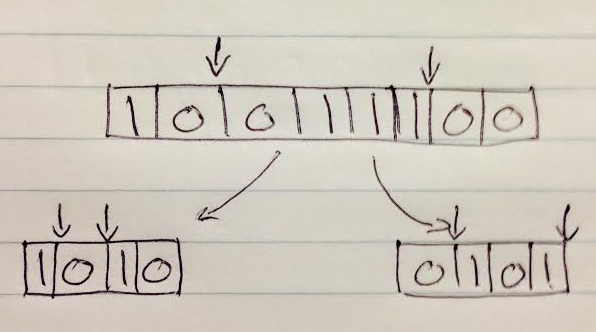
\includegraphics[width=0.6\textwidth]{pictures/bit_vector_split.png}
    \caption{When nodes inherit their bit vector ranges from their parent, it can become obvious if the entire subtree is contained within the range of $[y_1, y_2]$ or falls without the range.}
    \label{fig:bitvectorsplit}
\end{figure}


In order to make the rank query a constant time query, we create a partial rank sum list of the bit vector. This list contains the sum of the rank from $0$ to $i*\alpha$, where $\alpha$ is some constant. Using this partial rank sum list we can find the look up $rank(i*\alpha)$ and add the rank of the at most $\alpha$ next bits. Looking up the rank thusly takes $\mathcal{O}(1)$ time and requires $\mathcal{O}(n)$ space.

The actual coordinates of the points are only stored at the leaves which then takes up $\mathcal{O}(n)$ space. The rest of the tree only contains $\lg n$ levels of bit vectors of $n$ bits taking $\mathcal{O}(n \lg n)$ bits, $\mathcal{O}(n)$ words. Looking up the rank-space predecessor and successor of $x_1, x_2, y_1$ and $y_2$ using a simple binary search requires $\mathcal{O}(n)$ space and $\mathcal{O}(\lg n)$ time. Walking from the root to the $LCA$ requires $\lg n$ steps.

From here it requires $\mathcal{O}(\lg n + k*\lg n)$ query time to report $k$ points as results. An empty range will be detected already in the predecessor/successor lookup phase. If the lookup phase does not report an empty range, we proceed to use the algorithm. From the $LCA$ we are going to visit each leaf between $x^*_1$ and $x^*_2$ taking $\mathcal{O}(\lg n)$ time to visit each leaf.   

\begin{figure}[p]
    \centering
    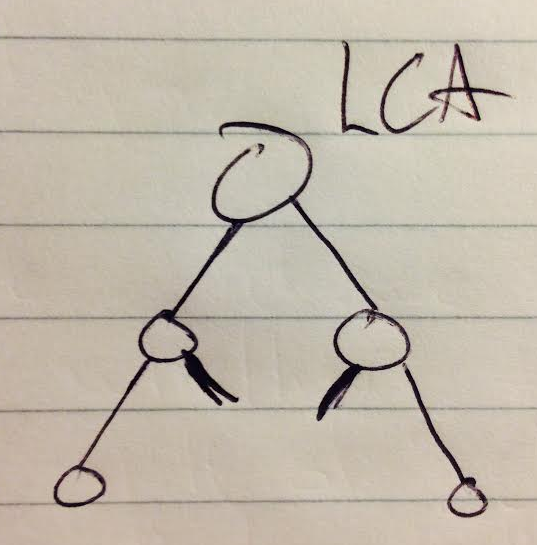
\includegraphics[width=0.6\textwidth]{pictures/LCA.png}
    \caption{Traversing left from the LCA, each right subtree contains x-coordinates between $x_1$ and $x_2$. Traversing right from the LCA the same holds for left subtrees.}
    \label{fig:LCA}
\end{figure}



\chapter{Primary Work}
\label{ch:primarywork}
\epigraph{``My name?'' said the old, and the same distant sadness came into his face again. He paused. ``My name,'' he said, ``is Slartibartfast.''}{---\textup{Douglas Adams}, Hitchhiker's Guide to the Galaxy}


This chapter will introduce the Simple Range Search and Original Range Search data structures. The Original Range Search data structure by \citet{chanetal} is a tree-like data structure with auxillary data structures. It has a space complexity of $\mathcal{O}(n)$ and a supports search queries in $\mathcal{O}(\lg\lg n + (1+k)\cdot\lg^\epsilon n)$ time, where $k$ is the amount of results reported and $\epsilon$ is an arbitrarily small constant greater than $0$.

The Simple Range Search data structure is a simplification of the Original Range Search and therefore they have the same underlying data structure. The Simple Range Search data structure has some different auxillary data structures and fewer of them. The data structure has a space complexity of $\mathcal{O}(n)$ and supports search queries in $\mathcal{O}(\lg n + (1+k)\lg^\epsilon n)$ time. Going forward,\emph{ORS} will be used as shorthand for \emph{Original Range Search} and \emph{SRS} will be used as shorthand for \emph{Simple Range Search}.


The SRS data structure has a time complexity of $\mathcal{O}(\lg n + (1+k)\cdot \lg^\epsilon n)$ which is greather than the time complexity of the ORS data structure with $\mathcal{O}(\lg \lg n + (1+k)\cdot \lg^\epsilon n)$. However, the SRS data structure is far more simple - both in code and the auxilary data structures used. The difference between the running time constant hidden in $\mathcal{O}(\lg \lg n)$ and $\mathcal{O}(\lg n)$ is far greater than the difference between $\lg \lg n$ and $\lg n$. This makes the SRS data structure faster than the ORS data structure in practice.

\vspace{4mm}

Each section will start with a \emph{preliminaries} subsection. This subsection will describe some of the auxiliary data structures used in the section. As in Chapter~\ref{ch:relatedwork}, the main data structures in this chapter are output-sensitive and static.

\section{Simple Range Search}
\label{sect:simple}

This section will introduce the primary work of this thesis. It will show how the SRS data structure is built and how range reporting is done using the data structure. The data structure uses $\mathcal{O}(n)$ space and supports search queries in $\mathcal{O}(\lg n + (1+k)\cdot \lg^\epsilon n)$ time. This is the same space complexity as the kd-tree. The query time is different in that $\mathcal{O}(\lg n)$ is smaller than $\mathcal{O}(\sqrt{n})$, but there is a cost of $\mathcal{O}(\lg^\epsilon n)$ per point reported. 

The SRS data structure relies heavily on the \emph{ball-inheritance} data structure. The ball-inheritance structure is a tree with $n$ labelled balls at the root. In $\lg n$ steps it will distribute the balls from the root of the tree to $n$ leaves in the tree. Solving the ball-inheritance problem is to follow a ball from any given node to its leaf. We formally define the problem below in section~\ref{ssect:ballinheritance}. Succint rank queries are an important part of data structure, playing a key role in solving the \emph{ball-inheritance problem}.

The SRS and ORS data structures supports search queries in a manner similar to the range tree. A balanced binary search tree is used to locate the subtrees which is fully contained in $[x_1, x_2]$. From here the range tree uses balanced binary search trees or fractional cascading to locate which of those points are in $[y_1, y_2]$, while the SRS and ORS data structures uses the ball-inheritance structure to decode the y-ranks to actual points.


\subsection{Preliminaries}

\subsubsection{Rank Space Reduction}
Given $n$ points from a universe $U$, the rank of a given point in a sorted list of points is defined as the amount of points which preceed it in the list. Given two points $a,b \in U: a < b$ \emph{iff} $rank(a) < rank(b)$. Expanding this concept to 2 dimensions we have a set $P$ of $n$ points on a $U \times U$ grid. We compute the \emph{x-rank} $r_x$ for each point in $P$ by finding the rank of the x-coordinate among all the x-coordinates in $P$. The \emph{y-rank} $r_y$ finds the rank of y-coordinate among all of the y-coordinates in $P$. Using \emph{rank space reduction} on $P$, a new set $P^*$ is constructed where $(x,y) \in P$ is replaced by $(r_x(x), r_y(y)) \in P^*$. Given a range query $q = [x_1, x_2] \times [y_1, y_2]$, a point $(x,y) \in P$ is found within $q$ \emph{iff} $(r_x(x), r_y(y))$ is found within $q^* = [r_x(x_1), r_x(x_2)] \times [r_y(y_1), r_y(y_2)]$. Computing the set $P^*$ from $P$ using rank space reduction, $P^*$ is said to be in rank space. While the $n$ points could be represented by $\lg U$ bits in $P$, they can now be represented by $\lg n$ bits in $P^*$ with $\lg n \ll \lg U$ when $n \ll U$ which saves memory. Given $n$ points from $U$ we can translate them to rank space by inserting them in an array $A[1..n]$ and sort $A$. A point's index in $A$ is now its rank. In order to translate a search query $q = [x_1, x_2]$ to rank space, we will look up the successor of $x_1$ in $A$ and the predecessor of $x_2$ in $A$. The indices of these two points delimits the search query in rank space. The array $A$ acts as a mapping to and from rank space. When a rank space reduction has been applied and there exists an array $A[1..n]$ mapping the elements to and from rank space, the algorithms used will only use RAM operations on integers of $\mathcal{O}(\lg n)$ bits.

\subsubsection{Predecessor search using binary search}
In order to find the rank space successor or rank space predecessor of a point, a binary search is used on a sorted array of points. This data structure uses $\mathcal{O}(n)$ space and have a query time of $\mathcal{O}(\lg n)$. By locating the first key in the array that is greater than or equal to the search query, the index of that key is the \emph{rank space successor}. Similarly, by locating the last key that is smaller in the array, the index of that key is the \emph{rank space predecessor}.



\subsubsection{Succint rank queries}
\label{sssect:succintrank}
Consider an array $A[1..n]$ with elements from some alphabet $\Sigma$. Given an index $i$ in the array, we can report how many elements in $A[1..i]$ are equal to $A[i]$. This is called a \emph{rank query}. We want to be able to compute a rank query in constant time using a data structure of $\mathcal{O}(n \lg \Sigma)$ bits. In order to do this, checkpoints are created. For each character in the alphabet $\Sigma$, the checkpoint contains the number of times that character appears in $A[1..i]$, where $i$ is the checkpoint location. Such a checkpoint takes up $\mathcal{O}(\Sigma \lg n)$ bits of space. By placing the checkpoints $\Sigma \lg n$ entries apart of each other, all of the checkpoints use $\mathcal{O}(\frac{n}{\Sigma \lg n} \cdot \Sigma \lg n) = \mathcal{O}(n)$ bits of space.

Each entry in $A$ contains a character from the alphabet $\Sigma$. At $A[i]$ we also store the amount of times the character at $A[i]$ occurs since the last checkpoint. This is a smaller number and can be stored using $\mathcal{O}(\lg (\Sigma \lg n))$ bits per entry in $A$. This is because we only need $\lg x$ bits to store a number which has a maximum value of $x-1$. This approach fits the required space bound if $\Sigma \geq \lg^\epsilon n$, because there $\Sigma$ will dominate the complexity. Hence, storing $n$ entries uses $\mathcal{O}(n\cdot\lg(\Sigma \lg n)) = \mathcal{O}(n\cdot\lg\Sigma)$ bits. Working under the word-RAM model of computation, we are able to pack the $n$ integers into $n\cdot\lg m$ bits, where $m$ is the maximum number which needs to be stored.

%For smaller alphabets, another scheme is used. Checkpoints are still stored at every $\Sigma \lg n$ positions. These are now called major checkpoints. In addition to this, minor checkpoints are added. These minor checkpoints are added at every $\lg \lg n$ positions and store the amount of times each character is seen since the last major checkpoint. These minor checkpoints take up $\mathcal{O}(\Sigma \lg \lg n)$ bits each. $A[i]$ now stores the character from the alphabet $\Sigma$ and how many times that character occurs since the last minor checkpoint. In order to answer the rank query, a query to the last major checkpoint and the last minor checkpoint has to be made. Given that $\Sigma \lg \lg n \leq \sqrt{\lg n} \cdot \lg \lg n$, the array entries holding the amount of times $A[i]$ is seen since the last minor checkpoint fits into $\mathcal{O}(\sqrt{\lg n} \cdot \lg^2 \lg n)$ bits. Therefore it is possible to store these array entries in plain form, and with the help of a precomputed table of $n^{\mathcal{O}(1)}$ space we can answer rank queries between minor checkpoints in constant time. \todo{Plain form?} \todo{rephrase} \todo{Maybe only need large alphabet +  bit vector. Then can leave out complicated multilevel}\todo{SE NOTER FOR CHANGES TIL DENNE BID}

%\noindent \textbf{Ball Inheritance Problem.} Given a perfect binary tree with $n$ leaves, we want to distribute $n$ labelled balls which appear in an ordered list at the root to the leaves in $\lg n$ steps. \todo{Rephrase}. The list of balls at a given node will inherited by its children with each child receiving the same amount of balls. Each level of the tree contains the same amount of balls. Eventually each ball reaches a leaf of the tree and each leaf will contain exactly one ball. The identity of a given ball is a node and the index of the ball in that nodes list. The true identity, the information the ball contains, only lies in the leaf. The \emph{ball-inheritance problem} is to track a ball from a given node to a leaf and report the identity of the leaf. \\


\subsubsection{Ball Inheritance}
\label{ssect:ballinheritance}
The input to the ball-inheritance problem is a perfect binary tree with $n$ leaves and $n$ labelled balls at the root. The balls have been distributed from the root to the leaves in $\lg n$ steps. All balls are mapped to distinct leaves and follow the path from the root to that leaf. Following this path from a node to its child, we say that a ball is inherited by that child. The balls at the root are contained in an ordered list, and they will retain this order at all internal nodes. Each node thus has an associated list of those balls going through it\todo{passing through, going through - thus? those eller which?}. The level of a node is defined to be the height of the node from the leaves. The root has the highest level, while each node is one level smaller than its parent. The leaves are at level $0$. Each level of the tree contains the same amount of balls, and at level $i$ each node contains $2^i$ balls. Eventually each ball reaches a leaf of the tree and each leaf will contain exactly one ball. A ball can be identified by a node and the index of the ball in the list of that node. Given the identity of a ball at any level, it is possible to follow this ball down the tree to a leaf. The goal is to track a balls inheritance from a given node to a leaf and report the identity of the leaf. We call the identity of the leaf the \emph{true identity} of a ball. 

\subsection{Solving the ball-inheritance problem} 
\label{ssection:solving-ball}

Consider an input to the ball-inheritance problem, i.e. a perfect binary tree with $n$ leaves and $n$ balls following root-to-leaves path. At level $m$, each node has a bit vector $A_v[1..2^m]$ used to indicate which child-node a ball is inherited by: If $A_v[i]$ is $0$ it means that the ball at index $i$ in that node's list is inherited by the left child and $1$ means that it is inherited by the right child. The identity of a ball is a node and an index into the list of that node. Given a node $v$ and an identity of a ball, we can now calculate the ball's identity in the child node which inherits the ball. The node can answer the query $rank_v(k) = \Sigma_{i \leq k} A_v[i]$. If a ball is inherited by the right child node its new identity at that node is $rank_v(i)$ because that is how many $1$'s that preceed it in the current node, and thus the number of balls inherited by the right child that preceeds the ball in the ball-ordering.. If a ball is inherited by the left child node the new identity is then $i-rank_v(i)$. With this information it is possible to traverse down the tree following a ball from any given node to a leaf. There are $n$ balls per level represented by the bit vectors of the nodes on that level. Each level in the tree uses $\mathcal{O}(n)$ bits to store the bit vectors. This adds up to $\mathcal{O}(n \lg n)$ bits, or $\mathcal{O}(n)$ words in all. This trivial solution to the ball-inheritance problem uses $\mathcal{O}(\lg n)$ query time, given that it follows a ball $\mathcal{O}(\lg n)$ steps down to its leaf. The rank function is a constant time query as described in section~\ref{sssect:succintrank} about succint rank queries.


\subsubsection{Faster Queries}
\label{ssection:fasterqueries}

In the solution above, a bit vector is an array with entries from the alphabet $\Sigma = \{0,1\}$, where each entry is used to indicate whether a left or right child has been chosen to inherit a given ball. By expanding the alphabet we can point to the children's children, $\Sigma = \{0,1,2,3\}$, the children's children's children, $\Sigma = \{0,1,2,3,4,5,6,7\}$, and so forth. Expanding the alphabet will use $\mathcal{O}(n \lg \Sigma)$ bits per level. Storing a pointer for each ball from level $i$ to level $i+\Delta$ increases the storage space by $\Delta$ bits per ball, but also enables the ball to be inherited by $2^\Delta$ descendants. By expanding the alphabet the query time can be lowered since it is possible to take bigger steps down the tree. Just like with a parent-to-child step, bigger steps are supported by succint rank queries. In order to determine the identity of a ball $b$ at $\Sigma$ levels below, we need to know the destination node and how many balls before $b$ chose the same destination node. Using succint rank queries to determine the rank of a ball $\Sigma$ levels down is thus a constant time query.

Using this concept, we pick $B$ such that $2 \leq B \leq m$, where $m = \lg n$ is the height of the tree. All levels that are a multiple of $B^i$ expand their alphabet such that the balls can also reach $B^i$ levels down. If a target level does not exist, the ball points to its leaf. We need at most visit $B$ levels that are multiple of $B^i$ before reaching a level that is multiple of $B^{i+1}$, making it possible to jump down the tree with bigger and bigger steps.

% $\Sigma^{\lg_B \lg n}_i \frac{\lg n}{B^i} \cdot \mathcal{O}(B^i) = \mathcal{O}(\lg n \cdot \lg_B \lg n)$ 
Storing the expanded alphabets at each level that is a multiple of $B^i$ costs $B^i$ bits per ball. The total cost is then 
\begin{align*}
  \sum\limits_{i=1}^{\lg_B \lg n} \frac{\lg n}{B^i} \cdot \mathcal{O}(B^i) = \mathcal{O}(\lg n \cdot \lg_B \lg n)
\end{align*}


\noindent bits per ball, summed over all levels. With $n$ balls, this is $\mathcal{O}(n \lg_B \lg n)$ words of space with query time of $\mathcal{O}(B \lg_B \lg n)$. If we pick a $B \geq \lg^\epsilon n$ we can reduce $\lg_B \lg n$ to $\lg_{\lg^\epsilon n} \lg n = \frac{1}{\epsilon}$. Thus, the space complexity for the ball-inheritance data structure is $\mathcal{O}(\frac{1}{\epsilon} \cdot n) = \mathcal{O}(n)$ words of space. By picking $B = \lg^{\epsilon / 2} n \geq \lg \lg n$ we can upper bound the query time as follows:
\begin{align*}
  \mathcal{O}(B \lg_B \lg n) &= \mathcal{O}(B \lg \lg n) = \mathcal{O}(\lg^{\epsilon /2} n \cdot \lg \lg n)\\
  &= \mathcal{O}(\lg^{\epsilon / 2} n \cdot \lg^{\epsilon / 2} n) = \mathcal{O}(\lg^\epsilon n)
\end{align*}

\noindent The ball-inheritance problem can thus be solved in $\mathcal{O}(\lg^\epsilon n)$ time using $\mathcal{O}(n)$ words of space for an arbitrary small constant $\epsilon > 0$.
\todo{Det er fordi $\lg_B \lg n$ er det største $i$ som beskriver $B^i \leq \lg n$ }

\subsection{Solving range reporting}

Recall from section ``range trees'' that a range tree had a 1-d binary tree over the x-coordinates and an auxiliry data structure to look up the y-coordinates of fully included nodes. The range reporting of the SRS data structures acts just like that. There is a 1-d range tree over the x-coordinates. When a fully included node is found from the least common ancestor of $x_1$ and $x_2$, we use the ball-inheritance structure as our auxiliary data structure to decode the location of the leaf by using the rank of the y-coordinate. So in essence, the range tree and SRS data structure is quite alike, just with a different auxiliary data structure. \todo{Omskriv til en meget bedre intro - hvor meget af det du fortæller her bliver først forklaret om lidt? Skal det også omskrives?}

Consider a perfect binary tree with $n$ leaves. The root contains $n$ points in $2$-d rank space. The elements in the ball-inheritance structure are points, so the words \emph{ball} and \emph{point} can be used interchangeably. The $n$ balls at the root of the tree are sorted by their y-rank. When distributing the balls for inheritance, a node will give both its children half of its balls: the lower half sorted by the x-rank to its left child and the upper half by x-rank to its right child. The order of the balls in a child node will be the same as the parent node. The actual coordinates of the balls are only stored at the leaves. This is how the ball-inheritance data structure was described in the previous section. The ball distribution has been specified. With this distribution, some facts about the tree can be stated. We know that the x-coordinates of the balls in the leaves are sorted from left to right - smallest to highest. The way the balls are distributed from the root, the x-coordinates are responsible for the inheritance path. Because the nodes are sorted by their y-rank in the root node and that they keep this order, the balls in a node list at any given node is ordered by their y-rank. These two facts will be used to solve the range reporting.

\noindent Since the actual coordinates of the points are only stored once, this data structure uses linear space. \\

Given a range query $q = [x_1, x_2] \times [y_1, y_2]$ the rank successors of $x_1$ and $y_1$ and the rank predecessors of $x_2$ and $y_2$ are looked up. We know that a range query can be translated to a rank space query. We call these $\hat{x}_1, \hat{y}_1, \hat{x}_2$ and $\hat{y}_2$. We now have our query $q$ in rank space: $\hat{q} = [\hat{x_1}, \hat{x_2}] \times [\hat{y_1}, \hat{y_2}]$. We use $\hat{x}_1$ and $\hat{x}_2$ to find the least common ancestor of $\hat{x_1}$ and $\hat{x_2}$, $LCA(\hat{x}_1, \hat{x}_2)$. The subtree rooted at this node contains at least all the points with an x-coordinate between $x_1$ and $x_2$. \\

At the root of the SRS data structure we mark the positions of $\hat{y}_1$ and $\hat{y}_2$ on the bit vector. This range indicates the balls lying within the range of $[y_1, y_2]$. We will denote the range of $[\hat{y_1} \hat{y_2}]$ marking the balls at node $v$ which has a y-coordinate in $[y_1, y_2]$ for $ \Gamma_v$\todo{Fjern det, hvis du ikke kommer til at bruge det}. Furthermore, $i_v$ and $j_v$ will denote this range in the bit vector of the node $v$. When searching for points lying within this range, a node will update this range to fit its children. The updated range at the left child $l$ will be $i_l = i_v - rank_v(i_v)$ and $j_l = j_v - rank_v(j_v)$. The updated range at the right child $r$ will be $i_r = rank_v(i_v)$ and $j_r = rank_v(j_v)$. This is the same way the rank query was used in section \ref{ssection:solving-ball}. Now instead of just following a given ball, we keep track of a range of balls. This concept is seen on figure~\ref{fig:bitvectorsplit}. \\

Traversing from the root to the $LCA$, this y-range will be updated accordingly. We know the positions of the leaves containing $\hat{x}_1$ and $\hat{x}_2$ so we can traverse from the $LCA$ down to each of them. Traversing to $\hat{x}_1$, the first stop is the left child of the $LCA$. From here, each time a node selects its left child as the path to $\hat{x}_1$ we know that the subtree contained in the right child only contains points with x-coordinates between $x_1$ and $x_2$. Symmetrically, the same applies when going right from the $LCA$: Each time a node selects a right child on the path to $\hat{x}_2$ the subtree contained in the left child only contains points between $x_1$ and $x_2$. Such a subtree is said to be fully contained. When a subtree is fully contained, we also say that the node at which the subtree is rooted is fully contained. This concept is seen on figure \ref{fig:LCA}. This is the same concept used with the range tree. \\

Each time a fully contained node $v$ is found, we want to follow all the balls lying in the range of $\Gamma_v$ from the root of the subtree rooted at $v$ to their leaves. This is exactly what the solution to the ball-inheritance problem provides: We are given a list of ball identities and want to find which leaf stores the actual coordinates of the point we are looking for. Finding the coordinates of a ball takes $\mathcal{O}(\lg^\epsilon n)$ time per ball. The $\mathcal{O}(\lg^\epsilon n)$ describes how many jumps are needed from a node to a leaf.

\begin{figure}[h]
    \centering
    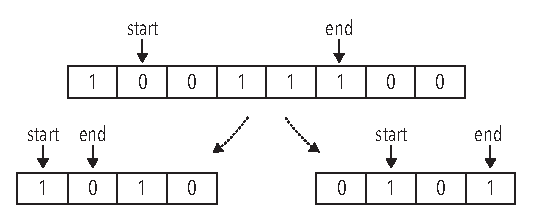
\includegraphics[width=0.95\textwidth]{pictures/bit_vector_split2.eps}
    \caption{Example of nodes inheriting their bit vector ranges from their parent.}
    \label{fig:bitvectorsplit}
\end{figure}


%The data structure is utilized as follows:
%\begin{enumerate}
%    \item Use a binary seach to find the rank space predecessors and successors of $x_1$, $y_1$, $x_2$ and $y_2$. At this point the algorithm will terminate if either rank space range is empty.
%    \item From $LCA(\hat{x}_1, \hat{x}_2)$, both $\hat{x}_1$ and $\hat{x}_2$ will be visited. The range y-rank range found in step $1$ will be updated from the root to this $LCA$ and updated from the $LCA$ to $\hat{x}_1$, $\hat{x}_2$ and all the subtrees between them.
%    \item Each time a fully included subtree is visited, we determine which balls falls within the y-range and use the ball-inheritance structure to travel to its leaf. When a leaf is visited, its actual coordinates will be reported back as a result.
%\end{enumerate}

The actual coordinates of the points are only stored at the leaves which then takes up $\mathcal{O}(n)$  words of space. The rest of the tree contains $\lg n$ levels of bit vectors of $n$ bits taking $\mathcal{O}(n \lg n)$ bits, $\mathcal{O}(n)$ words. Looking up the rank-space predecessor and successor of $x_1, x_2, y_1$ and $y_2$ using a simple binary search at the root requires $\mathcal{O}(n)$ space and $\mathcal{O}(\lg n)$ time. Summing it up, the entire data structure uses $\mathcal{O}(n)$ words of space. 

Walking from the root to the $LCA$ requires $\mathcal{O}(\lg n)$ steps. Walking to $\hat{x}_1$ and $\hat{x}_2$ from the $LCA$ requires $\mathcal{O}(\lg n)$ steps each. Visiting each of the $k$ leaves in the subtrees between $\hat{x}_1$ and $\hat{x}_2$, storing the points which will be reported as a result, takes $\mathcal{O}(k \cdot \lg^\epsilon n)$ time. \todo{omformuler} This adds up to $\mathcal{O}(\lg n + (1+k)\cdot\lg^\epsilon n)$ query time to report $k$ points as results. \todo{Måske tilføje en sætning eller to}

\begin{figure}[h]
    \centering
    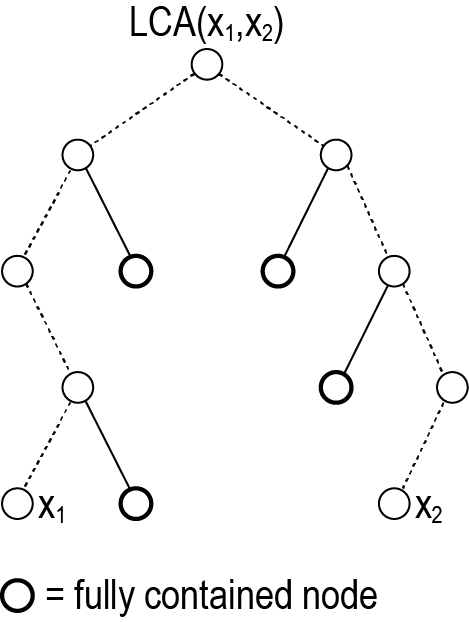
\includegraphics[width=0.6\textwidth]{pictures/LCA2.png}
    \caption{Traversing left from the LCA, each right subtree contains x-coordinates between $x_1$ and $x_2$. Traversing right from the LCA the same holds for left subtrees. Dotted line represent the path from the lowest common ancestor of $x_1$ and $x_2$ to $x_1$ and $x_2$}
    \label{fig:LCA}
\end{figure}


\section{Original Range Search}
\label{sect:original}

This section describes the ORS data structure. While the theoretical work of this thesis is a simplification of this data structure, the ORS can also be viewed as an extension of the SRS. The ORS data structure will \underline{not} be implemented, but serves as a theoretical background for the SRS. The main property the SRS and ORS share is that the underlying data structure is the ball-inheritance data structure and solving the range reporting heavily relies on solving the ball-inheritance problem.

Utilizing the ball-inheritance structure, \citet{chanetal} propose a theoretically better solution for orthogonal range search queries than the one of the Simple Range Search data structure: 
\begin{customthm}{2.1}\label{theorem21}
for any $2 \leq B \leq \lg^\epsilon n$, we can can solve $2$-d orthogonal range reporting in rank space with $\mathcal{O}(n \lg_B \lg n)$ space and $(1+k)\mathcal{O}(B \lg \lg n)$ query time.
\end{customthm}

In this section some supporting data structures will be introduced. Then we will show how the ball-inheritance is used in conjunction with these data structures to find the points within a search query $q = [x_1, x_2] \times [y_1, y_2]$.

\subsection{Preliminaries}

\subsubsection{Range minimum queries}
In order to find the smallest element in a range, a succint data structure will be used. This data structure can solve the \emph{range minimum query} problem and will be referred to as RMQ. 
Consider an array $A$ with $n$ comparable keys, this succint data structure allows finding the index of the minimum key in the subarray $A[i,j]$. \citet{fischer} introduces a data structure which solves this problem in $2n + \mathcal{O}(n)$ bits of space with constant query time. The construction requires that the array is ordered, which we will see fits into our scheme. Note that $\mathcal{O}(n)$ is less than the bits needed to store $A$. Thus, only the index of the minimum key in $A[i,j]$ can be returned, not the actual key.


\subsubsection{Rank space predecessor search}
In order to look up the rank space predecessor of a given coordinate, another succint data structure will be used. This data structure has a worse space complexity than the RMQ and a bigger query time.
Given a sorted array $A[1..n]$ of $\omega$-bit integers, predecessor search queries in $\mathcal{O}(\lg \omega)$ time is supported using $\mathcal{O}(n \lg \omega)$ bits of space with \emph{oracle access} to the entries in the array. Since $\mathcal{O}(n \lg \omega)$ bits of space is not enough to store $n$ $\omega$-bit integers, the data structure will only store part of each $n$ elements and defer the look-up operation to an \emph{oracle machine}. For this purpose a Patricia trie \cite{morehaste} is used to store some parts of the $n$ $\omega$-bit integers and find which entries in the array $A$ which has to be looked up by the oracle machine. The oracle machine is some data structure that, given an index $i$, can return $A[i]$. 

\subsubsection{Finding the lowest common ancestor}
In the Simple Range Search, the lowest common ancestor of $x_1$ and $x_2$ was found by following the path from the root of the tree to both $x_1$ and $x_2$. The last node both paths shared was then the lowest common ancestor. This way of finding the lowest common ancestor takes $\mathcal{O}(\lg n)$ time which is too big for the Original Range Search.
In order to look up the lowest common ancestor of $x_1$ and $x_2$ in constant time, we are going to look at the binary representation of $x_1$ and $x_2$. First we look at $x_1 \oplus x_2$. The number of zero bits from to the start to the first one bit describes the amount of nodes the two paths have in common. We denote this number $b$. This will tell us to look on level $\lg n - b$. The number that the first $b$ bits of $x_1$ describes is the identity of the lowest common ancestor of $x_1$ and $x_2$ on level $\lg n - b$. Modern machines have an instruction for finding the most significant set bit of a number in constant time. Thus, the lowest common ancestor of $x_1$ and $x_2$ can be found in constant time.


\subsection{Solving range reporting}

With a solution to the ball-inheritance problem, \citet{chanetal} propose the following: 
\begin{customlem}{2.4}\label{lemma24}
if the ball inheritance problem can be solved with space $S$ and query time $\tau$, $2$-d range reporting can be solved with space $\mathcal{O}(S+n)$ and query time $\mathcal{O}(\lg \lg n + (1+k) \tau)$.
\end{customlem}


The ball distribution scheme of this data structure is the same as the simplified range search of section \ref{ssection:solving-ball}. Having distributed the $n$ points from the root to the leaves, additional data structures are required in order to answer the range queries. For each node in the tree that is a right child a range minimum query structure is added. The indices are the y-rank and the keys are the x-rank that the given node contains. A range maximum query structure is added to all the nodes which are left children. Each data structure uses $2n + \mathcal{O}(n)$ bits, making it $\mathcal{O}(n)$ bits per level of the tree and $\mathcal{O}(n \lg n)$ bits in all - i.e. $\mathcal{O}(n)$ words of space. \\

In order to support predecessor (and successor) search for the y-rank in the data structure, the rank space predecessor search data structure is added to the tree. This data structure works on an array of the y-ranks, which is already sorted. The points in rank space of $\mathcal{O}(\lg n)$ bits will use $\mathcal{O}(n \lg \lg n)$ bits per level, with $\omega = \lg n$, and $\mathcal{O}(n \lg n \lg \lg n)$ bits in all, which is $\mathcal{O}(n \lg \lg n)$ words. In order to reduce this to linear space we will only place this predecessor search structure at levels which are multiples of $\lg \lg n$. When using the predecessor search from the lowest common ancestor of $\hat{x}_1$ and $\hat{x}_2$, $LCA(\hat{x}_1, \hat{x}_2)$, we go up to the closest ancestor node which has a predecessor structure in order to perform the search there. Searching takes $\mathcal{O}(\lg \lg n)$ time plus $\mathcal{O}(1)$ queries to the ball-inheritance structure. The ball-inheritance structure is exactly the oracle machine that the rank space predessecor search needs: At any given node the balls are sorted by their y-rank and given the identity (the index) of a ball at that node, it can look up the y-coordinate by decoding the y-rank to a leaf storing a point. Using the ball-inheritance structure we walk at most $\lg \lg n$ steps down while translating the ranks of $y_1$ and $y_2$ to the right and left child of $LCA(\hat{x}_1, \hat{x}_2)$. 

The reason why this structure is necessary for the y-ranks and not the x-ranks, is because of the way the points have been distributed in the ball-inheritance tree: From left to right, the leaves have x-rank $1,2,..n$ so we can easily locate a given range in the x dimension, but in order to keep track of the y-dimensional range we need to follow the balls down the ball-inheritance structure. Adding this structure to each $\lg \lg n$ level saves us from going all the way from the root down to the $LCA$. \\

\noindent In order to use this data structure to report points in the range of $q = [x_1, x_2] \times [y_1, y_2]$ we follow these steps:
\begin{enumerate}
  \item We find the rank space successor of $x_1$ and the rank space predecessor of $x_2$. We call them $\hat{x}_1$ and $\hat{x}_2$. We use these to find the lowest common ancestor of $\hat{x}_1$ and $\hat{x}_2$, $LCA(\hat{x}_1, \hat{x}_2)$. This is the lowest node in the tree whose subtree contains at least all the points between $x_1$ and $x_2$. By knowing $\hat{x}_1$ and $\hat{x}_2$, finding the lowest common ancestor is a constant time operation.   
  %\item As in step $1$ where we found the rank space of the x-coordinates, we find the rank space coordinates of the y-coordinates, $\hat{y}_1$ and $\hat{y}_2$, inside the left and right child of $LCA(\hat{x}_1, \hat{x}_2)$. We are only interested in the rank of $y_1$ and $y_2$ among the points stored in the left and right subtree of $LCA(\hat{x}_1, \hat{x}_2)$. This step is precisely what the rank space predecessor structure mentioned above supports.
  \item From the least common ancestor of $x_1$ and $x_2$, we walk at most $\lg \lg n$ steps up to find the nearest parent with a predessecor search structure for the y-rank. We then translate $y_1$ and $y_2$ into rank space coordinates. We then walk down to the LCA again while maintaining the $\hat{y_1}$ and $\hat{y_2}$ at each step. The rank space coordinates are then translated into both the left and right child of the LCA. At each of the two children of the least common ancestor, this range indicates which balls have a y-coordinate between $y_1$ and $y_2$, i.e. which leaves that stores a point with a y-coordinate between $y_1$ and $y_2$. This step is illustrated on figure~\ref{fig:orstep2}
  \item We now descend into the right child of $LCA(\hat{x}_1, \hat{x}_2)$ and use the range minimum query structure at this node to the find the index $m$ (the y-rank) of the point with the smallest x-rank in the range $[\hat{y}_1, \hat{y}_2]$. The y-rank of a point at a node is exactly the identity of the ball going to the leaf storing the point. Knowing the identity of the ball we can use the ball-inheritance structure to follow the path to the leaf to find the actual x-coordinate of the point. If the x-coordinate is smaller than $x_2$ we return the point as a result and recurse into the ranges of $[\hat{y}_1, m-1]$ and $[m+1, \hat{y}_2]$ in order to find more points. Otherwise we terminate. When this is done we apply the same concept to the left child of $LCA(\hat{y}_1, \hat{x}_2)$ using the range maximum query to find points above $x_1$.
\end{enumerate}


\begin{figure}[h]
    \centering
    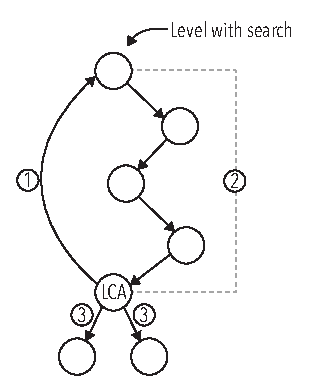
\includegraphics[width=0.65\textwidth]{pictures/ors_step2.eps}
    \caption{Illustration of how step $2$ of the OBIS works.}
    \label{fig:orstep2}
\end{figure}




%\todo{Insert figure to conceptually show we are working our way out from the inside} We look at figure~\ref{fig:orstep2} for an idea of how step $2$ works. \circled{1} shows how we go to the nearest parent with predecessor search structure to find $\hat{y_1}$ and $\hat{y_2}$. \circled{2} shows how $[\hat{y_1}, \hat{y_2}]$ is translated into the corresponding range for the LCA by translating them one level at a time. \circled{3} We now translate $[\hat{y_1}, \hat{y_2}]$ from the LCA into its left child. \circled{4} We now translate $[\hat{y_1}, \hat{y_2}]$ from the LCA into its right child. \todo{Skal omformuleres hvis det skal med i den endelige version}

%\todo{Indsæt figur der viser at vi går fra LCA op til nærmeste parent og så ned i begge børn} At figure~\ref{fig:orsearchfigure} we can see how the ORS operates in step $3$ when finding results in the children of the LCA. $LCA_x$ describes the line between the points in the left child and the points in the right child. In the left child, given a range $[m_1, m_2]$ we find the index $m_p$ of the point with the largest x-coordinate in that range. If it is within our search query, we accept it and recurse into the ranges of $[m_1, m_p -1]$ and $[m_p+1, m_2]$ to find more points. At the right child we look for the points with smallest x-coordinates instead of biggest.\todo{Skal omformuleres hvis det skal med i den endelige version}

The time complexity of step $3$ depends on the use of the ball-inheritance structure. The time to traverse this structure is dependent on the improvements made in \ref{ssection:solving-ball}. An empty range will result in two queries, one query to each child of $LCA(\hat{x}_1, \hat{x}_2)$. In the worst case the amount of queries to the ball-inheritance structure will be twice the number of results reported plus one. Each time a result is found, a recursion is made to both the left and right subrange of that result. If one of the sides constantly fails to find a result, at most two queries are made for each result found. For the final result found, two ranges are recursed into which reports no results.

Conceptually, $LCA(\hat{x}_1, \hat{x}_2)$ describes a point between $x_1$ and $x_2$, more precisely a point with an x-coordinate higher than all the points in the left child and higher than all the points in the right child. Step $3$ selects points that are in the range of $[y_1, y_2]$ moving outwards from the point of $LCA(\hat{x}_1, \hat{x}_2)$, always picking the point closest to $LCA(\hat{x}_1, \hat{x}_2)$ in its decreasing y-range. We can see an example of how step $3$ works on figure~\ref{fig:orsearchfigure}. Looking at the right child of the figure, the leftmost point in the range $[\hat{y_1}, \hat{y_2}]$ will be found first. If that point has an x-coordinate less or equal to $x_2$ it will be part of the result. Then we recurse into the ranges $[p_7, p_8]$ and $[p_9, p_9]$. When the leftmost point in a range has an x-coordinate which is greater than $x_2$ then all other points in that range will also have an x-coordinate greater than $x_2$. Thus, the recursion in that range stops. Symmetrically, same applies for the left child of the least common ancestor.

Going back to Lemma $2.4$, we see that the time complexity fits: $\mathcal{O}(\lg \lg n)$ time is used for the predecessor search and $\mathcal{O}((1+k)\tau)$ time is used for walking from the children of the $LCA$ to the leaves solving the ball inheritance problem for the $k$ results.


\begin{figure}[h]
    \centering
    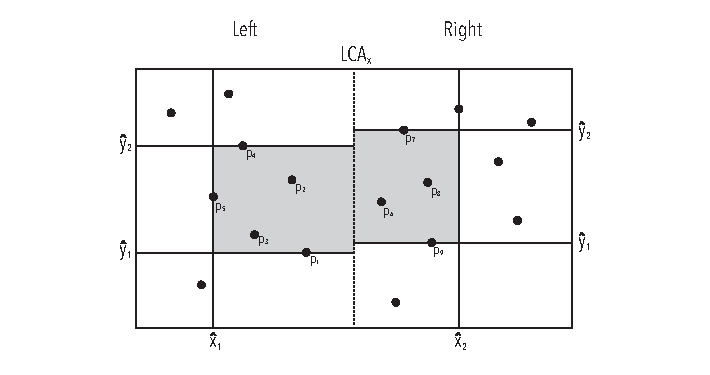
\includegraphics[width=0.95\textwidth]{pictures/ors_step3.eps}
    \caption{Illustration of how step $3$ of the OBIS works. The dotted line divides the points in the left and right child of the least common ancestor.}
    \label{fig:orsearchfigure}
\end{figure}
\clearpage


\section{Summary}
\label{sect:summaryprim}

The SRS and ORS data structures both uses $\mathcal{O}(n)$ words of space. Both relies heavily on the ball-inheritance data structure in order to store and retrieve the actual coordinates of points. Both data structures supports retrieval of points through the ball-inheritance data structure in $\mathcal{O}(\lg^\epsilon n)$ time. The main difference between the SRS data structure and the ORS data structure is the rest of the query time: $\mathcal{O}(\lg n)$ for the SRS and $\mathcal{O}(\lg \lg n)$ for the ORS. The ORS data structure relies on more auxillary data structures of greater complexity than the SRS data structure. Thus, the theoretical running time of a range query to ORS is smaller than a range query to the SRS. In practise, it is safe to assume a range query to the SRS is faster than a range query to the ORS. With much more code to be executed and using more advanced auxillary data structures, the running time constant hidden in $\mathcal{O}(\lg \lg n)$ can be quite large. Also,  the factor between $\lg n$ and $\lg \lg n$ is not that big. Given a very large dataset of $2^{64}$ elements as input, $\lg 2^{64} = 64$ and $\lg \lg 2^{64} = 6$, which has a factor $\sim10$ difference. \\


Both the SRS data structure and the kd-tree uses $\mathcal{O}(n)$ words of space. This is an attractive property when working on the RAM. Like all the main data structures mentioned in this thesis, the kd-tree and SRS data structure are output-sensitive. A range query to the kd-tree has a running time of $\mathcal{O}(\sqrt{n}+k)$ and a range query to the SRS data structure has a running time of $\mathcal{O}(\lg n + (1+k)\cdot\lg^\epsilon n)$. When $n$ grows, $\mathcal{O}(\sqrt{n})$ grows at a faster rate than $\mathcal{O}(\lg n)$. For each point reported as a result from a range query to the SRS data structure there is a cost of a factor $\mathcal{O}(lg^\epsilon n)$ while each point reported as a result from a range query to the kd-tree has a cost of a factor $\mathcal{O}(1)$. The $\mathcal{O}(\sqrt{n})$ running time of the range query to the kd-tree is due to a pessimistic idea that a range query will overlap, but not fully include, a lot of regions in the kd-tree. So dependent on the shape of the range query to the kd-tree, the running time can vary a lot. The $\mathcal{O}(\lg n)$ part of the range query to the SRS data structure is due to the initial binary search and to follow the path from the root of the tree to $x_1$ and $x_2$. Thus, the running time of a range query to the SRS data structure will behave more stable (fluctuate less) than the running time of a range query to the kd-tree. 


\todo{Kan man sige noget en sammenligning af de to worst-cases? At den ene er bedre end den anden og det sætter en bedre upper bound?}

Another aspect of range querying is testing for emptiness. When testing for emptiness, a range query can stop the moment a single result is found since it is a test with the binary outcome of ``yes'' or ``no''. The SRS data structure will be able to determine emptiness of a range query with no ball-inheritance queries. Hence, an emptiness query to the SRS data structure can be checked in $\mathcal{O}(\lg n)$ time. The initial binary search to find the rank space query might indicate that there are no points in $[x_1, x_2]$ or $[y_1, y_2]$. If the initial binary search does not indicate an empty range, the range query will continue normally. The moment a query to the ball-inheritance structure is made, the range is not empty and the emptiness test can report back without doing the actual ball-inheritance query. An emptiness query to the kd-tree can checked in $\mathcal{O}(\sqrt{n})$ time. The same argument as before applies: The query might overlap with a lot of regions which it does not fully contain, and within those regions none of the points are within the range. On the other hand, when a fully contained region is found the emptiness test can report back with a result. Given a range query $[x_1, x_2] \times [y_1, y_2]$, the SRS data structure will have a more stable running time for its emptiness test than the kd-tree. The running time of a query made to the kd-tree will fluctuate a lot depending on the shape of the query.

\todo{Ting du skal huske at have med i dette kapitel: Decode y-rank i stedet for at slå op i søgetræ. Range-tree imod ball-inheritance}
\todo{Balls per level vs balls per node - hvordan skal det introduceres (og hvor). Rank af bolde i node (per node)}
\todo{Har jeg nævnt at $\lg^\epsilon n$ er antal hop?}
\todo{Ret lige lidt i emptiness test}


\part{Practical}

\chapter{Implementation}

\section{Language}

In order to implement the $SRS$ data structure and the kd-tree, C++11 was used. C++11 is a recent release of C++. C++11 combines the advantages of a modern programming language with the stability and support of a mature language which have been around for more than three decades. C++11 was chosen for several reason: It does not have garbage collection, it is a high level language with support for low level operation and contains libraries for everything needed in this project. The chrono header gives access to a high resolution clock to meassure time. The vector class of the standard template library is very straight-forward container to work with and the underlying structure is a continuous block of memory making it ideal for cache purposes. The algorithm header gives access to convenience functions for generating and sorting data.

\section{Design choices}

The theory describes the ball inheritance data structure as a binary tree with internal node and leaves. Each node then has a ball inheritance list to show which ball was inherited by which child. In practise all the ball inheritance lists per level are merged together to one, resulting in $\lg n$ ball inheritance lists in all. Instead of being an actual entity, a node is just defined as which level it is from, where on that levels list its ball inheritance list starts and how many balls its list holds. Since each ball only uses a single bit per level there would have been a lot of space wasted when nodes only held two or four balls in their ball inheritance lists. By having one list per level we can pick one data type to work without independent of how many balls needs to be stored per node. std::uint32\_t \todo{hvordan skriver jeg det pænt?} was chosen in this case. It is an unsigned fixed width integer type of $32$ bits.


Skriv om hvordan det virker med enkelte hop. Vi har en look-up til 16 bits. Vi har en sum for hvert 32 bits. At 0 bare er komplementar af 1 når vi tæller.

\chapter{Analysis}
\label{ch:analysis}
\epigraph{``The trouble with writing fiction is that it has to make sense, whereas real life doesn't"}{--- \textup{Iain M. Banks}}

The purpose of this chapter is to compare the BIS data structure to the kd-tree. We are going to perform a variety of experiments on the BIS data structure and the kd-tree in order to determine the run-time properties of both, mainly looking at when the BIS data structure performs better than the kd-tree.


When performing the experiments, random data will be generated and given as input to the data structures. Both data structures will be given the same random data. This way they operate on the some data and the comparison will be fair. The random data is generated by making two lists, $X$ and $Y$ with the integers $[0,n-1]$ and shuffling them both randomly. The $n$ points given to the data structures as input are found by taking the $i$th entry of both $X$ and $Y$ and generating a point with those coordinates. This ensures that all x-coordinates are unique and all y-coordinates are unique. When running a specific test, different data sets will be generated and given as new input to the data structures such that a test is not only performed on a single data set. The different experiments will check how the shape of a given search query impacts the running time of the query to the data structures. When the shape and size of the search query has been determined, the search will performed with a different displacement on the x-axis and y-axis such that the queries are performed all over the data structure and not only in a best-case or worst-case position. The search query is performed a lot of times and then the average time per query is returned. \\

We are mainly going to focus on two different kinds of experiments. First we are going to test how a search query shaped like a square performs in both the BIS data structure and the kd-tree. This type of query will be good for the kd-tree since it will get to fully include many regions. In the second test the configuration of the search query is going to one where the worst-case scenario for the kd-tree happens. It will cover the entirety of the search area in a thin slice either in a vertical or horizontal direction. In the third section we are going to look closer at how much better the search query to the BIS data structure compares to the search query to the kd-tree when the search query is a vertical or horizontal slice and $k \leq 200$. The limit of $200$ is chosen because it is small and a reasonable upper bound on the amount of results for human interaction.\\

The experiments have been performed on data structures with data sets of size $2^{\lg n}$ where $\lg n = [17,25]$. $17$ was chosen as the smallest because it would still be big enough to show something interesting on the graphs. $25$ was chosen because the current initialization of the BIS data structure requires a bit of work and thus takes up nearly all of the main memory. Future work includes an idea for a faster and less memory requiring setup phase.\\

In all the test we have chosen $B = \lceil \frac{1}{2}\lg^{\frac{1}{3}} n \rceil$. Recall from section~\ref{ssection:fasterqueries} that we must have $B = \Omega(\lg^\epsilon n)$ to obtain linear space. Thus, we have chosen $\epsilon = \frac{1}{3}$. Section~\ref{ssection:fasterqueries} also states that $B$ is responsible for the big jumps in the ball inheritance structure: where the jumps should be placed and how big they should be. Unless otherwise stated the graphs in this chapter show results from a BIS data structure configured with $B = \lceil \frac{1}{2}\lg^{\frac{1}{3}} n \rceil$.


The experiments were performed on a machine with an Intel i7-3770 CPU with 3.40GHz and with $32$ GB RAM. The machine was running Ubuntu 14.04.2 LTS with clang version 3.4. The machine was provided by MADALGO.



\section{Square search queries}
\label{sect:squares}

This section will show the running time of square search queries to both data structure. With this configuration we expect to see that kd-tree performs better than the BIS data structure. We are interested in seeing just how much worse the BIS data structure performs. 

\subsection{Setup}
The kd-tree has a query time of $\mathcal{O}(\sqrt{n}+k)$. The $\sqrt{n}$ part is based on a pessimistic notion that an edge of a query will pass through the entire search area of the kd-tree. This is not always the case. We also note that when $k > \sqrt{n}$, $k$ will dominate the expression and thus the query time will be linear in the output size. In order to fairly compare the running time of a search query to both data structure, we are going to generate queries finding the points within a rectangle with the area of $\sqrt{size}\cdot\sqrt{n} \times \sqrt{size}\cdot\sqrt{n}$ where size will increase. As previously described, this search query will be made with random displacements in order to query arbitrary places in the structures. So given two random numbers $x$ and $y$ a query will be $q = [x, x+\sqrt{size}\cdot\sqrt{n}] \times [y, y+\sqrt{size}\cdot\sqrt{n}]$. A query of this shape will not invoke the worst-case scenario for the kd-tree and will thus give an idea of how the BIS data structure performs in contrast to the kd-tree under circumstances where the kd-tree performs well. \\

The points generated for the data structures lie in the range of $[0,n-1] \times [0,n-1]$, which gives an area of $n^2$. If the search query has an area of $A$, each point has a $\frac{A}{n^2}$ chance of being in that search query. With $n$ points we thus expect to find $n\cdot \frac{A}{n^2}$ points in a search query with the area of $A$. In this test we set $A = \sqrt{n}\cdot\sqrt{size}\times\sqrt{n}\cdot\sqrt{size}$, where $n$ is constant to the data structure and $size$ will increase during the test. We then expect to find $n\cdot\frac{A}{n^2} = \frac{n\cdot n \cdot size}{n^2} = size$ points. This obviously depends a lot on how the points are distributed in that specific case. When generating $10$ different data sets for the data structures in the tests and picking the displacements for the search query at random each search, we will expect the average amount of points returned by the search query $q = [x, x+\sqrt{size}\cdot\sqrt{n}] \times [y, y+\sqrt{size}\cdot\sqrt{n}]$ to be $size$.

\subsection{Data}

On figure~\ref{fig:sqrt_17} and figure~\ref{fig:sqrt_25} we see that the running time of a query to the BIS data structures, for a fixed $n$, increases linear to the amount of points returned. This agrees with the theoretical running time of $\mathcal{O}(\lg n + k\cdot \lg^\epsilon n)$. The theoretical $\mathcal{O}(\lg^\epsilon n)$ is the worst-case amount of jumps from a any given node to a leaf. On figure~\ref{fig:sqrt_25} we notice that around $size\approx 150$ the graph changes its slope. The slope decreases which means that the running time per point decreases. This means that the average amount of jumps per point reported can change, but will naturally always be bounded by the worst-case of $\lg^\epsilon n$. Other factors may have a say in the change of slope as well. Some of these factors will be mentioned in section~\ref{sect:verthoriexp}.

\noindent As expected, the average amount of points reported from a lot of search queries with $q = [x, x + \sqrt{size}\cdot\sqrt{n}] \times [y, y + \sqrt{size}\cdot\sqrt{n}]$ were $size$ or $size-1$. When $\sqrt{size}\cdot\sqrt{n}$ is a floating point number it will be rounded down to the nearest integer. \\

The graphs on figure~\ref{fig:sqrt_17} and figure~\ref{fig:sqrt_25} show the time of a search query to the BIS data structure compared to the time of a search query to the kd-tree. The shape of the search query is a square. The variable $size$ increments in levels of $5$ per iteration of the test and will have a maximum of $\frac{\sqrt{n}}{2}$. The x-axis of the graphs describes the $size$ variable in the expression $A = \sqrt{n}\cdot\sqrt{size} \times \sqrt{n}\cdot\sqrt{size}$. Examining figure~\ref{fig:sqrt_17} we see that when the shape of the search query is a square, the search query to the kd-tree is always performing better than the search query to the BIS data structure. Looking closer at the figure we notice that while the search query to the BIS data structure performs worse, it is not that bad. At $size = 180$ we have window of size $\sqrt{2^{17}}\cdot\sqrt{180} \times \sqrt{2^{17}}\cdot\sqrt{180} = 4857.26 \times 4857.26$. The time to perform the search query on the BIS data structure at $size = 180$ is $15.9$ microseconds, while the search to the kd-tree takes $5.2$. This search query includes $180$ points. This is a relatively big query and the time to perform the search query on the BIS data structure is only a factor $3$ worse than the time of the search query on kd-tree.


% This can have something to do with the different ways the BIS data structure and the kd-tree behaves given a search query. The kd-tree uses the actual search query in its normal form, $[x_1, x_2] \times [y_1, y_2]$ and compares that with the region of each node the search encounters. The first things the BIS data structure does given a search is to translate it into rank space. In rank space we know precisely how many points are in $[\hat{x_1}, \hat{x_2}]$ and $[\hat{y_1}, \hat{y_2}]$ and thus the search query is dependent on how many points are in $[\hat{x_1}, \hat{x_2}]$ and $[\hat{y_1}, \hat{y_2}]$ rather than how big the search query is. \todo{Skriv om}

Examining figure~\ref{fig:sqrt_25} with $n = 2^{25}$ the largest search window has become quite large with a size of $\sqrt{2^{25}}\cdot\sqrt{2895} \times \sqrt{2^{25}}\cdot\sqrt{2895} = 311673 \times 311673$. The biggest window now returns $2895$ points. A search query with this size to the BIS data structure and the search query to the kd-tree has a factor $\frac{386}{24} = 16.1$ difference. This a quite big difference in the search time, but it is also a big search query.

It is obvious from the graphs that the kd-tree performs better when the search queries are square windows. The time of a search query to the BIS data structure grows linearly to the size of the window, just like a query to the kd-tree, but with a bigger slope. This means you will not run into an unexpected growth when asking for more points from the BIS data structure. \\

The biggest search query at $n = 2^{17}$ is $\sqrt{180}\cdot{n} \times \sqrt{180}\cdot\sqrt{n}$. We now fix $size = 100 \leq 180$ and see how the ratio between the search query to the BIS data structure and kd-tree will evolve when $n$ grows. We see this on figure~\ref{fig:factdiffsqrt100}. The graph is growing and thus the running time of a search query to the BIS data structure grows faster than same search query to the kd-tree when $n$ is growing. This is to be expected since we pay $\mathcal{O}(k\cdot\lg^\epsilon n)$ compared to $\mathcal{O}(k)$. The ratio grows from $2.3$ to $5.5$ when $\lg n$ grows from $17$ to $25$. This is not a huge increase in ratio taking into account that $n$ grows by a factor of $\frac{2^{25}}{2^{17}} = 2^8 = 256$.

\begin{figure}[h]
  \makebox[\linewidth][c]{
    \centering
    \begin{subfigure}[b]{0.68\textwidth}
        \centering
        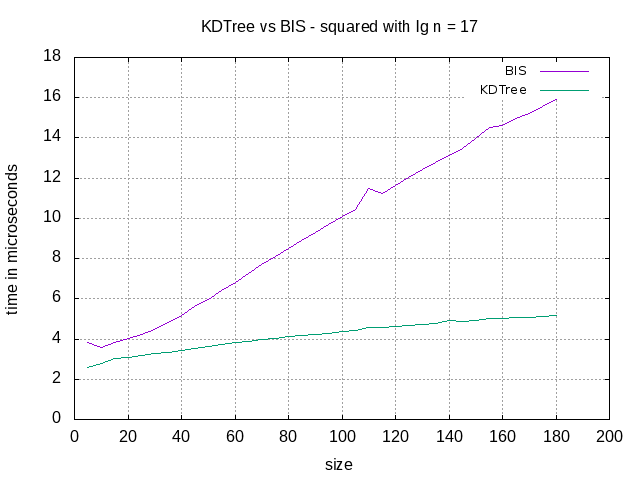
\includegraphics[width=0.99\textwidth]{pictures/analysis/sqrt_17.png}
        \caption{$n = 2^{17}$ with $\sqrt{n} = 362$.}
        \label{fig:sqrt_17}
    \end{subfigure}
    %\hfill
    \begin{subfigure}[b]{0.68\textwidth}
        \centering
        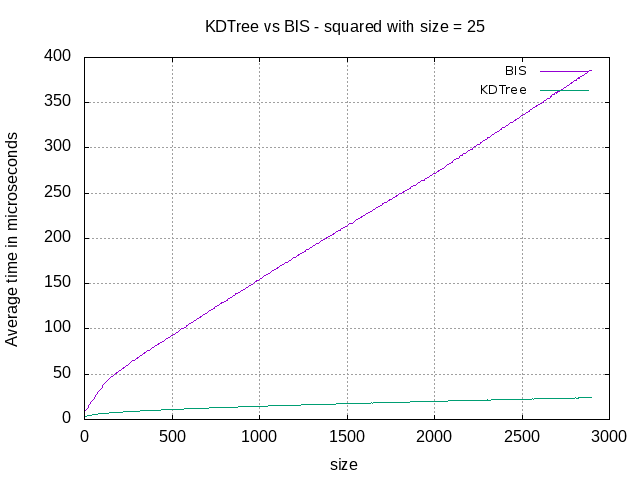
\includegraphics[width=0.99\textwidth]{pictures/analysis/sqrt_25.png}
        \caption{$n = 2^{25}$ with $\sqrt{n} = 5792$.}
        \label{fig:sqrt_25}
    \end{subfigure}
  }
    \caption{Square search on BIS and kd-tree.}
    \label{fig:sqrt_17_25}
  
\end{figure}

\begin{figure}[h]
    \centering
    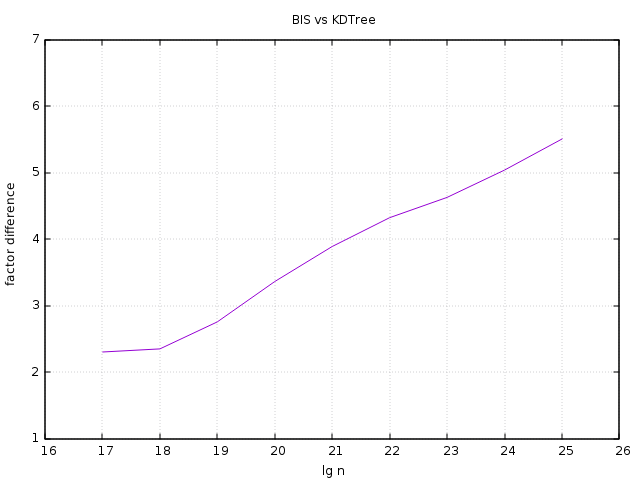
\includegraphics[width = 0.85\textwidth]{pictures/analysis/factor_difference_sqrtn_100.png}
    \caption{Ratio between a square query to the kd-tree and BIS data structure with constant $size = 100$. Ratio describes how much better the kd-tree performs.}\label{fig:factdiffsqrt100}
\end{figure}

\clearpage


\section{Vertical and horizontal slices}
\label{sect:slices}

In this section we are going to compare the performance of the BIS data structure and the performance of the kd-tree when the search query is in the shape of a \emph{slice}. We define a \emph{slice} to be a search query which covers the entirety of the search space in one dimension while only covering a small part of the search space in the other dimension. Since a slice is a search query with the form of either $q_h = [0, n-1] \times [y_1, y_2]$ or $q_v = [x_1, x_2] \times [0, n-1]$ we omit $[0, n-1]$ and define the \emph{size of the slice} to be $\left| y_2-y_1\right|$ or $\left|x_2-x_1\right|$. A slice which extends through the entirety of the x-dimension is called a \emph{vertical slice}. A slice which extends through the entirety of the x-dimension is called a \emph{horizontal slice}. Both the x-coordinates and y-coordinates of the points generated are unique which means that a slice of size $k$ will always return $k$ points as the result.

\subsection{Setup}

A search query to the kd-tree has a run-time of $\mathcal{O}(\sqrt{n}+k)$ and a search query to the BIS data structure has a run-time of $\mathcal{O}(\lg n + k \cdot \lg^\epsilon n)$. We expect the run-time of a slice to the BIS to be faster when $k$ is small. When $k$ grows the kd-tree will eventually become faster. When increasing the size of a slice, we expect the run-time of the two search queries to be roughly equal at $k \approx \frac{\sqrt{n} - \lg n}{\lg^\epsilon n - 1}$. This originates from $\sqrt{n} + k = \lg n + k \cdot \lg^\epsilon n \Leftrightarrow k = \frac{\sqrt{n} - \lg n}{\lg^\epsilon n - 1}$. We call this theoretical intersection point between the running times for $k_t$. The $\mathcal{O}(\lg^\epsilon n)$ bounds the amount of jumps needed to perform in order to find the identity of a leaf given the identity of a ball in the ball inheritance structure. $\lg^\epsilon n$ intuitively describes the amount jumps a ball uses to travel from a node to a leaf. Thus, in this analysis $\lg^\epsilon n$ will be the average amount of jumps per result, as measured by the results in the experiments. For example, if the ball-inheritance structure has used $10$ jumps to locate $4$ leaves, $\lg^\epsilon n = \frac{10}{4} = 2.5$. We use this measured $\lg^\epsilon n$ instead of the theoretical $\lg^\epsilon n$ because the theoretical is used to bound the amount of jumps, not count them. Thus, in $k_t$ we will let $\lg^\epsilon n$ describe the average amount of jumps taken by each point reported back as a result of the query, measured by the experiments.

Recall that the BIS data structure treats the two dimensions very differently. Given a rank space search query $\hat{q} = [\hat{x_1}, \hat{x_2}] \times [\hat{y_1}, \hat{y_2}]$, the search algorithm will find the least common ancestor of $\hat{x_1}$ and $\hat{x_2}$. From there, it will find the path to both $\hat{x_1}$ and $\hat{x_2}$ and all leaves between them will be in the range $[x_1, x_2]$. The search algorithm now has to determine which of these leaves contain a point with y-coordinate in $[y_1, y_2]$. This is done by using the ball inheritance structure from each of the fully contained nodes which were found on the path from the least common ancestor to $\hat{x_1}$ and $\hat{x_2}$.

This means that a horizontal slice and a vertical slice will be treated differently by the BIS data structure. The search query of a horizontal slice includes all x-coordinates of the search space, and thus the least common ancestor of $[\hat{x_1}, \hat{x_2}]$ will be the root of the tree. The path from the least common ancestor to $\hat{x_1}$ will only go left which means each level will have one fully contained node. The path from the least common ancestor to $\hat{x_2}$ will only go right, also yielding one fully contained node per level. The tests measure the difference in performance between the BIS data structure and the kd-tree when the search query is a slice. A slice will start out being very small, $k=5$. Thus, many of the fully contained nodes will have no ball inheritance work when the slice is a horizontal slice. As the slice grows, eventually more and more node will have one or more balls to follow. The amount of ball inheritance each node is responsible for varies a lot, and therefore the ball inheritance will become somewhat sporadic. But the nature of the ball distribution asserts that if node has two or more balls for ball inheritance, these balls will be right next to each other.

On the other hand we have the vertical slices. The vertical slice includes all y-coordinates of the search space, and thus the location of the least common ancestor of $[\hat{x_1}, \hat{x_2}]$ varies a lot dependent on the search query. But the nodes which are marked as fully contained on the path from the least common ancestor to $\hat{x_1}$ and $\hat{x_2}$ will all only contain leaves with points with y-coordinates in $[y_1, y_2]$ which means we have to do ball inheritance on all the balls belonging to fully contained nodes. Thus, the ball inheritance in vertical slices are much more batched together. Comparing a vertical and horizontal slice of the same size, the vertical slice will have good chances of being faster than the horizontal slice. With a least common ancestor closer to the leaves, the ball inheritance in the vertical slice will have to jump from a lower level than the ball inheritance in the horizontal and the balls are more batched together in the vertical. \\

We are going to look at how well the vertical and horizontal slices perform on both the BIS data structure and the kd-tree. We are interested in seeing how big the slices can become before the search query to the BIS data structure performs worse than the search query to the kd-tree. We are going to look at the vertical slices first. Below are some graphs showing the running time of a search query to both the BIS and the kd-tree dependent on the size of the slice. 

\subsection{Vertical slices}

Figure~\ref{fig:vert_17} and figure~\ref{fig:vert_25} show the performance of a search query to the BIS data structure compared to a search query to the kd-tree, where the search query is a vertical slice. Figure~\ref{fig:vert_17} shows that the BIS data structure is faster than the kd-tree up until the size of the slice is $200$. That is quite significant. Not only is the BIS data structure faster when $k \leq 200$, but at $k = 100$ it is approximately twice as fast as the kd-tree. There is a sudden change in the slope of the graph at around $k \approx 250$ which will be addressed in section~\ref{sect:verthoriexp}. On figure~\ref{fig:vert_25} we see that the BIS data structure is faster than the kd-tree up to a size of $4660$. That is big query. At $k = 100$ the BIS data structure is $27$ times faster than the kd-tree. At $k = 200$ the BIS data structure is $14$ times faster than the kd-tree. These are pretty significant differences in performance. \\


\begin{figure}[h]
  \makebox[\linewidth][c]{
    \centering
    \begin{subfigure}[b]{0.68\textwidth}
        \centering
        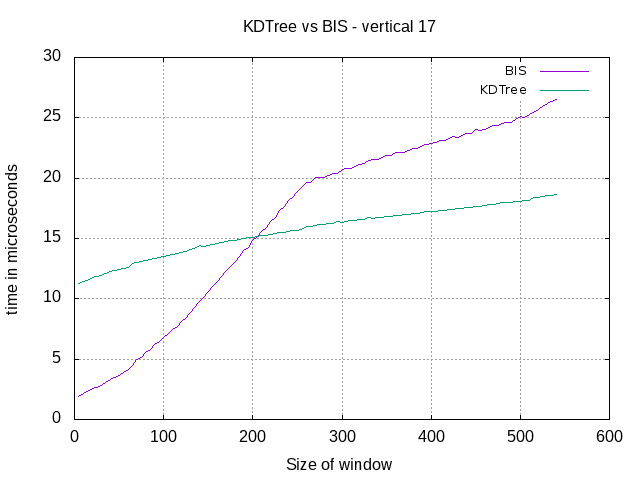
\includegraphics[width=0.99\textwidth]{pictures/analysis/vert_17.png}
        \caption{$n = 2^{17}$}
        \label{fig:vert_17}
    \end{subfigure}
    %\hfill
    \begin{subfigure}[b]{0.68\textwidth}
        \centering
        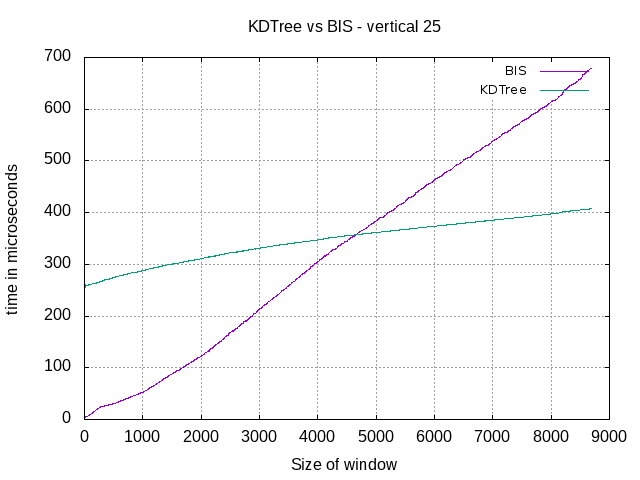
\includegraphics[width=0.99\textwidth]{pictures/analysis/vert_25.png}
        \caption{$n = 2^{25}$}
        \label{fig:vert_25}
    \end{subfigure}
  }
    \caption{Vertical slice on BIS and kd-tree.}
    \label{fig:vert_17_25}
  
\end{figure}


We just pointed out that the graphs on figure~\ref{fig:vert_17} intersect at $k = 200$ and the graphs on  figure~\ref{fig:vert_25} intersect at $k = 4660$. Figure~\ref{fig:vert_intersection} shows the size ($k$) of the slice at the point of intersection between the running-time of a search to the BIS and the kd-tree for each $n$ tested. Recall the theory above where it was described how the intersection point should theoretically be $k_t = \frac{\sqrt{n} - \lg n}{\lg^\epsilon n - 1}$. Figure~\ref{fig:vert_theory} shows $\frac{k_m}{k_t}$, where $k_m$ is the amount of results measured by the experiments. The graph is plotted using $\lg^\epsilon n$ as the average jumps per result as measured by the experiments. We want this graph to as close to a flat line as possible. It does not really matter where on the y-axis the flat line lies, because both the numerator and denominator of $k_t$ has hidden constants in the O-notation. We notice that the graph lies steadily around $1$ meaning that it is a stable relationship. Figure~\ref{fig:vert_intersection} has a exponential tendency. That is to expected since the x-axis is $\lg n$ which means that $n$ grows by a factor of $2$ each step on the x-axis and then the point of intersection between the two running times increases by approximately $\sqrt{2}$. This is because of the $\mathcal{O}(\sqrt{n})$ part from the running time of a search query to the kd-tree. Obviously, $\sqrt{n}$ grows by a factor of $\sqrt{2}$ when $n$ grows by a factor of $2$, which is exponential. A search query in the shape of a slice is the worst-case scenario for the kd-tree.

\begin{figure}[h]
  \makebox[\linewidth][c]{
    \centering
    \begin{subfigure}[b]{0.68\textwidth}
        \centering
        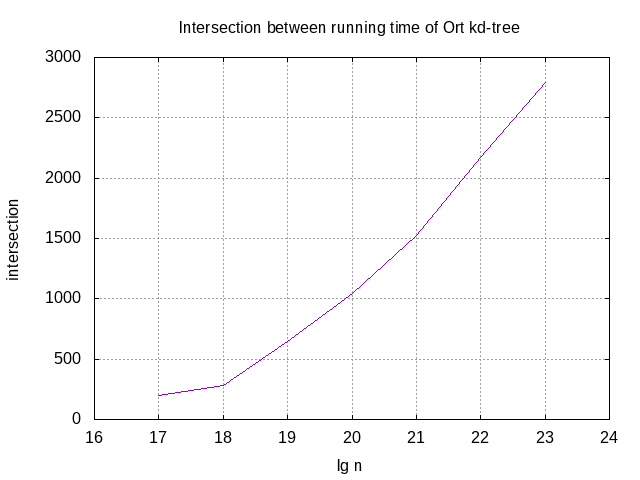
\includegraphics[width=0.99\textwidth]{pictures/analysis/vert.png}
        \caption{Point of intersection between BIS and kd-tree.}
        \label{fig:vert_intersection}
    \end{subfigure}
    %\hfill
    \begin{subfigure}[b]{0.68\textwidth}
        \centering
        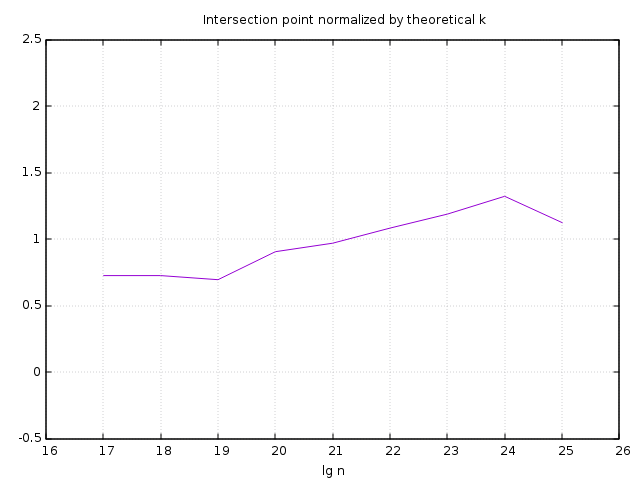
\includegraphics[width=0.99\textwidth]{pictures/analysis/vert_theory.png}
        \caption{Point of intersection normalized by theoretical $k$}
        \label{fig:vert_theory}
    \end{subfigure}
  }
    \caption{Vertical slice on BIS and kd-tree.}
    \label{fig:vert_intersection_and_theory}
  
\end{figure}
\clearpage


\subsection{Horizontal slices}

We are now going to look at the graphs for the horizontal slices. Recall that when a search query is a horizontal slice, the least common ancestor will be the root of the tree. In $[\hat{x_1}, \hat{x_2}]$, $\hat{x_1}$ will be the leftmost leaf and $\hat{x_2}$ will be the rightmost leaf. From the root to $\hat{x_1}$ and $\hat{x_2}$ there will many fully contained nodes, $2$ per level to be exact, which means there will be many different nodes performing small amount of balls inheritance look-ups. The y-coordinates of the points are uniformly distributed. Thus, unlike the vertical shape, we cannot say anything as definitively about where the ball-inheritance takes place. We are going to take a closer at this in section~\ref{sect:verthoriexp}. \todo{Kan skrives pænere - flyt eller slet. Det forvirrer nok mere end det hjælper. Det er jo ``setup''}


Figure~\ref{fig:hori_17} and figure~\ref{fig:hori_25} show the performance of a search query to the BIS data structure compared to a search query to the kd-tree, where the search query is a horizontal slice. Figure~\ref{fig:hori_17} shows that the BIS data structure is faster than the kd-tree until the size of the slice becomes $125$. While not as good as the vertical slice, it is still a decent size. At $k = 100$ the BIS data structure is only a factor $1.2$ faster than the kd-tree. On figure~\ref{fig:hori_25} we see that the BIS data structure is faster than the kd-tree up until $k = 2290$. At $k = 100$ the BIS data structure is $13$ times faster than the kd-tree, and at $k = 200$ it is $8$ times faster. Again, this is not as good as the vertical slice, but it is still quite significant. Given a query with $200$ results in a horizontal window, the BIS data structure outperforms the kd-tree by a factor of $8$. It is obvious for both the horizontal and the vertical slice, that the smaller the window, the better is ratio between the performance of the two data structures.


\begin{figure}[h]
  \makebox[\linewidth][c]{
    \centering
    \begin{subfigure}[b]{0.68\textwidth}
        \centering
        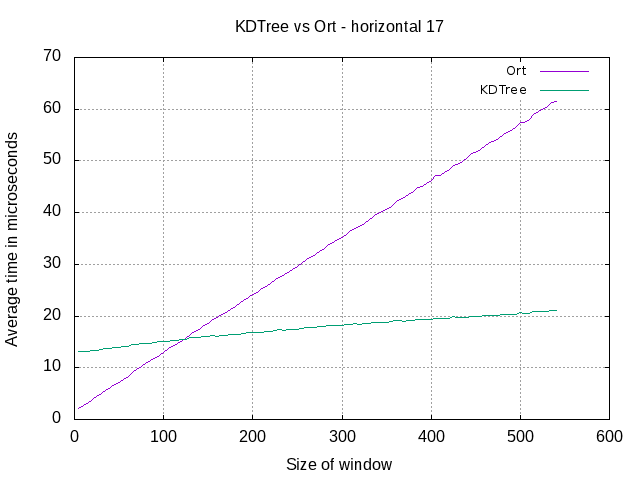
\includegraphics[width=0.99\textwidth]{pictures/analysis/hori_17.png}
        \caption{$n = 2^{17}$}
        \label{fig:hori_17}
    \end{subfigure}
    %\hfill
    \begin{subfigure}[b]{0.68\textwidth}
        \centering
        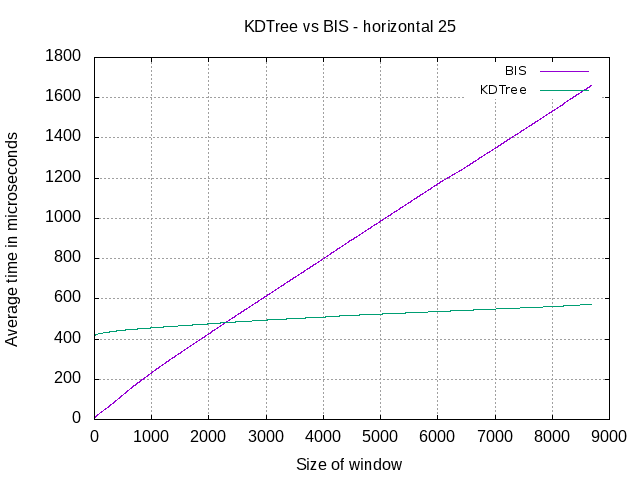
\includegraphics[width=0.99\textwidth]{pictures/analysis/hori_25.png}
        \caption{$n = 2^{25}$}
        \label{fig:hori_25}
    \end{subfigure}
  }
    \caption{Horizontal slice on BIS and kd-tree.}
    \label{fig:hori_17_25}
  
\end{figure}


Figure~\ref{fig:hori_intersection} shows the size ($k$) of the slice at the point of intersection between the running-time of a search to the BIS and kd-tree for each $n$ tested. Figure~\ref{fig:hori_intersection} is a little more messy than figure~\ref{fig:vert_intersection} which is a point we will address in section~\ref{sect:verthoriexp}. At figure~\ref{fig:hori_theory} the graph crosses above and below $1$, but keeps rather close to $1$ which is the point where the performance is as we would theoretically expect. Again, we are looking for a graph that is as flat as possible in order to show that is a stable relationship. In the big perspective, this graph certainly shows a stable relationship around $1$. Just as before, the $\lg^\epsilon n$ in $k_t$ is the average amount of jumps per result measured by the experiments. While the horizontal slice is not as good as the vertical slice, it is still very good. It definitely outperforms the kd-tree up to a good size.

\begin{figure}[h]
  \makebox[\linewidth][c]{
    \centering
    \begin{subfigure}[b]{0.68\textwidth}
        \centering
        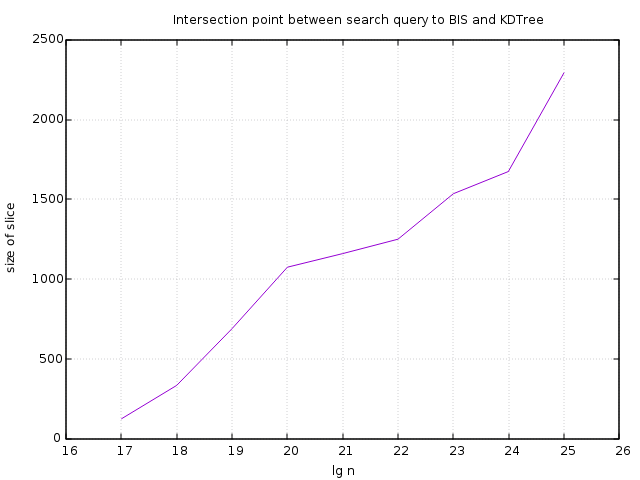
\includegraphics[width=0.99\textwidth]{pictures/analysis/hori.png}
        \caption{Point of intersection between BIS and kd-tree.}
        \label{fig:hori_intersection}
    \end{subfigure}
    %\hfill
    \begin{subfigure}[b]{0.68\textwidth}
        \centering
        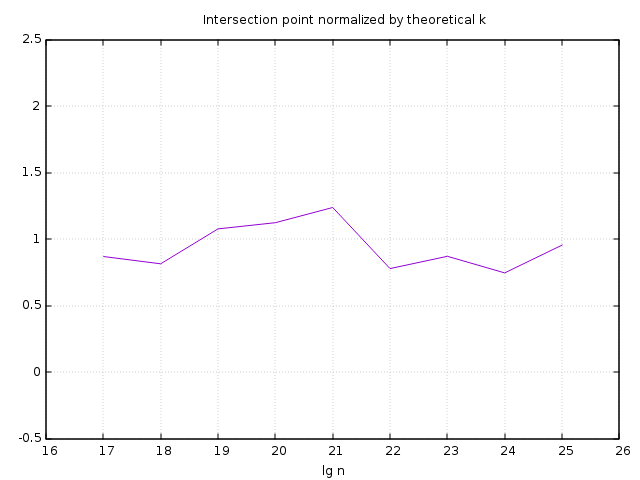
\includegraphics[width=0.99\textwidth]{pictures/analysis/hori_theory.png}
        \caption{Point of intersection normalized by theoretical $k$}
        \label{fig:hori_theory}
    \end{subfigure}
  }
    \caption{Horizontal slice on BIS and kd-tree.}
    \label{fig:hori_intersection_and_theory}
  
\end{figure}
\clearpage

\section{Slices with small $k$}
\label{sect:smallk}


In this section we are going to look at slices with $k\leq 200$. We will only focus on vertical slices. We are interested in seeing how much faster the BIS data structure is than the kd-tree when looking at amounts of results which seems reasonable to user interaction. Figure~\ref{fig:small_vert_17} figure~\ref{fig:small_vert_25} show the performance a search query to the BIS data structure compared to a search query to the kd-tree, where $k \leq 200$ for vertical slices.

\begin{figure}[h]
  \makebox[\linewidth][c]{
    \centering
    \begin{subfigure}[b]{0.68\textwidth}
        \centering
        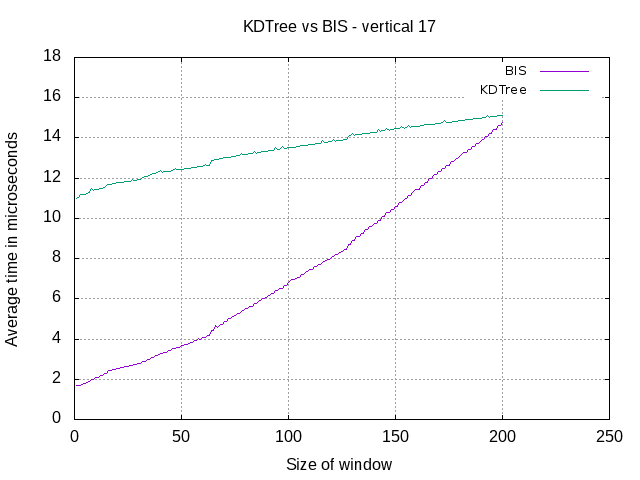
\includegraphics[width=0.99\textwidth]{pictures/analysis/smalls/vert_17.png}
        \caption{Data set of size $n=2^{17}$.}
        \label{fig:small_vert_17}
    \end{subfigure}
    %\hfill
    \begin{subfigure}[b]{0.68\textwidth}
        \centering
        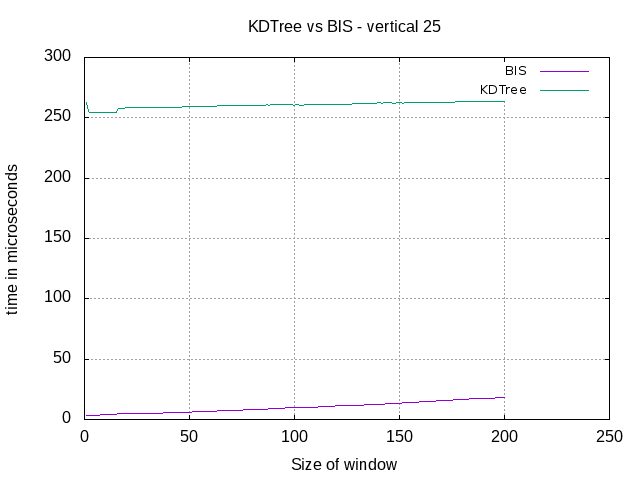
\includegraphics[width=0.99\textwidth]{pictures/analysis/smalls/vert_25.png}
        \caption{Data set of size $n=2^{25}$.}
        \label{fig:small_vert_25}
    \end{subfigure}
  }
    \caption{Vertical slice on BIS and kd-tree.}
    \label{fig:small_vert_17_25}
  
\end{figure}

The running time of a slice to the BIS data structure where $k \leq 200$ is noticeably better than the running time of a slice to the kd-tree. There is a great gap between the graph of the two running-times. The figures show that the BIS data structure always performs better when the size of the slice is below $200$. Seeing this tendency, we are then also interested in testing just how much better the BIS data structure performs. We are going to measure this by looking at the factor between the performance of the BIS data structure and the performance of the kd-tree. We see this on figure~\ref{fig:small_vert_fac_17} and figure~\ref{fig:small_vert_fac_25}. The ratios describes how much better the BIS data structure is than the kd-tree in terms of running time: Bigger is better. As mentioned in section~\ref{sect:slices}, the ratio between the performance of the BIS data structure and the kd-tree is strictly decreasing as the size of the slice is increasing. Thus, the smaller the slice, the bigger the ratio between performances of the data structures. 



\begin{figure}[h]
  \makebox[\linewidth][c]{
    \centering
    \begin{subfigure}[b]{0.68\textwidth}
        \centering
        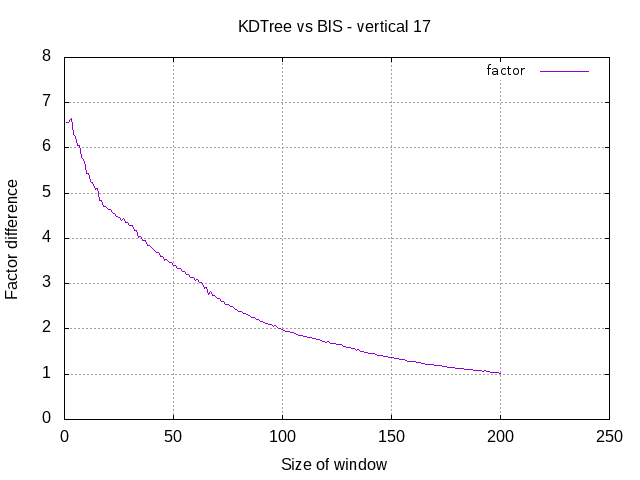
\includegraphics[width=0.99\textwidth]{pictures/analysis/smalls/vert_fac_17.png}
        \caption{Data set of size $n=2^{17}$.}
        \label{fig:small_vert_fac_17}
    \end{subfigure}
    %\hfill
    \begin{subfigure}[b]{0.68\textwidth}
        \centering
        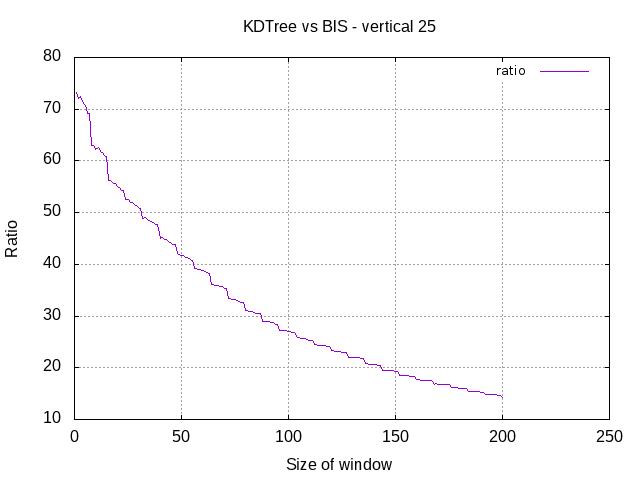
\includegraphics[width=0.99\textwidth]{pictures/analysis/smalls/vert_fac_25.png}
        \caption{Data set of size $n=2^{25}$.}
        \label{fig:small_vert_fac_25}
    \end{subfigure}
  }
  \caption{Ratio between running time of slice on BIS and kd-tree with fixed $n$.}
    \label{fig:small_vert_fac_17_25}
  
\end{figure}

Looking at figure~\ref{fig:small_vert_fac_17} and figure~\ref{fig:small_vert_fac_25} we notice that the ratio between the two running times at $size = 100$ increases from $2$ to $27$ as $n$ increases from $2^{17}$ to $2^{25}$. A factor of $27$ is the difference between the vertical slice to the BIS data structure and a vertical slice to the kd-tree with $size = 100$. With $size = 200$ the ratio between the two data structures increases from just above $1$ to $14$. A factor $14$ is a big difference. We see that when the size of the slice is constant and $n$ is growing, the ratio between a slice to the BIS data structure and the kd-tree increases. On figure~\ref{fig:small_vert_fac_25} we also notice that when $1 \leq k \leq 50$ the ratio is between $73$ and $42$. Thus, given a big data set and a small vertical slice the BIS data structure will significantly outperform the kd-tree. This fits well with the theory where the kd-tree has the worst-case of $\mathcal{O}(\sqrt{n})$ and the BIS data structure is more stable in respect to its shape. We will investigate this further.

Looking back to the section about the square windows we remember that a window with the dimensions $\sqrt{n}\cdot{size} \times \sqrt{n}\cdot\sqrt{size}$ is expected to return $size$ points as result. This was based on the area of area of the search query. Thus, we can rewrite the expression as follows: $\sqrt{n}\cdot{size} \times \sqrt{n}\cdot\sqrt{size} = \sqrt{n}\cdot\sqrt{n} \times \sqrt{size}\cdot\sqrt{size} = n \times size$. This is exactly what vertical or horizontal slice looks like. Thus, we know that these two types of queries are expected to return the same amount of points and we can therefore compare the square search query with a horizontal or vertical slice to see how much of an impact the shape of the search has for the BIS data structure. \\

We pick $size=\{50,100,150\}$ from both the square experiments and the slice experiments to see how changing the shape of the query affects the running time of the query to the BIS data structure. The graphs on figure~\ref{fig:all_50}, figure~\ref{fig:all_100} and figure~\ref{fig:all_150} show some similarities. The vertical slice is clearly the fastest. The horizontal slice performs worse than the vertical slice. The squared search query seems to be the worst-case scenario for the BIS data structure. But looking at only the squared search across the three graphs we see that it growing with a rather linear tendency. We would expect as much from the theory because if we fix $k$ in $\mathcal{O}(\lg n + k\cdot \lg^\epsilon n)$ we only have $\lg n$ and $\lg^\epsilon n$ growing. Since $\lg n$ increases by $1$ and $\mathcal{O}(lg^\epsilon n)$ is a bound for the amount of jumps performed, this ties rather well to the theory. Looking at these three graphs, we suspect that the square search is the worst case of a search query to the BIS data structure, while both the horizontal and vertical slice searches are special cases performing even better. Thus, when we fix $k$ and let $n$ grow, the time required to find $k$ points with a search query to the BIS data structure seems to be bound by the running time of the square search. 


\begin{figure}[h]
  \makebox[\linewidth][c]{
    \centering
    \begin{subfigure}[b]{0.68\textwidth}
        \centering
        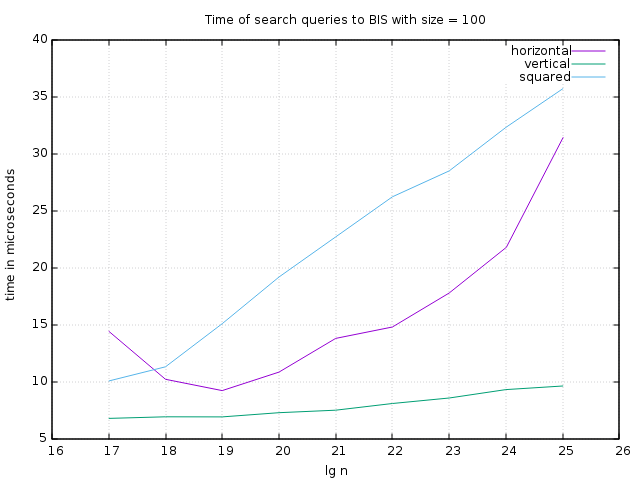
\includegraphics[width=0.99\textwidth]{pictures/analysis/smalls/all_100.png}
        \caption{Queries to the BIS data structure with $size=100$.}
        \label{fig:all_100}
    \end{subfigure}
    %\hfill
    \begin{subfigure}[b]{0.68\textwidth}
        \centering
        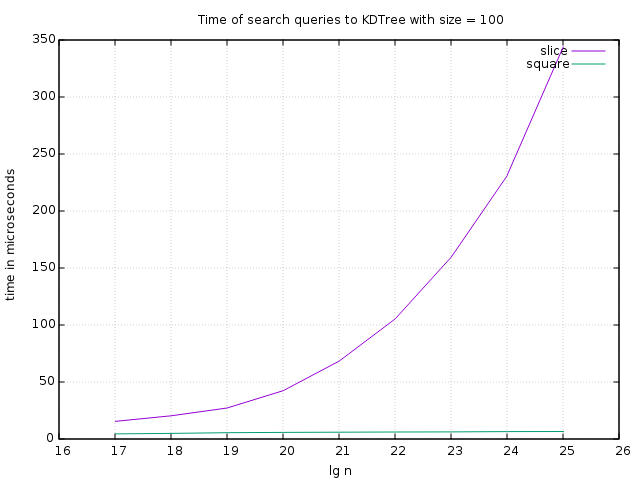
\includegraphics[width=0.99\textwidth]{pictures/analysis/smalls/all_kdtree_100_2.png}
        \caption{Queries to the kd-tree with $size=100$.}
        \label{fig:all_kdtree_100}
    \end{subfigure}
  }
  \caption{Comparison of shapes on BIS and KDtree.}
  \label{fig:all_100_and_kdtree}
  
\end{figure}

\begin{figure}[h]
  \makebox[\linewidth][c]{
    \centering
    \begin{subfigure}[b]{0.68\textwidth}
        \centering
        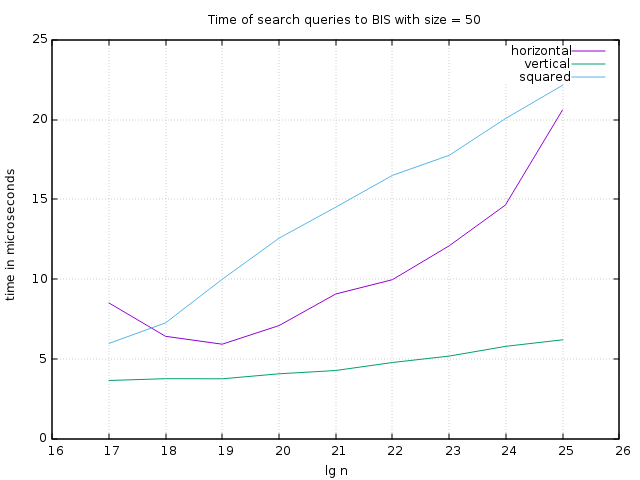
\includegraphics[width=0.99\textwidth]{pictures/analysis/smalls/all_50.png}
        \caption{Queries to the BIS data structure with $size=50$.}
        \label{fig:all_50}
    \end{subfigure}
    %\hfill
    \begin{subfigure}[b]{0.68\textwidth}
        \centering
        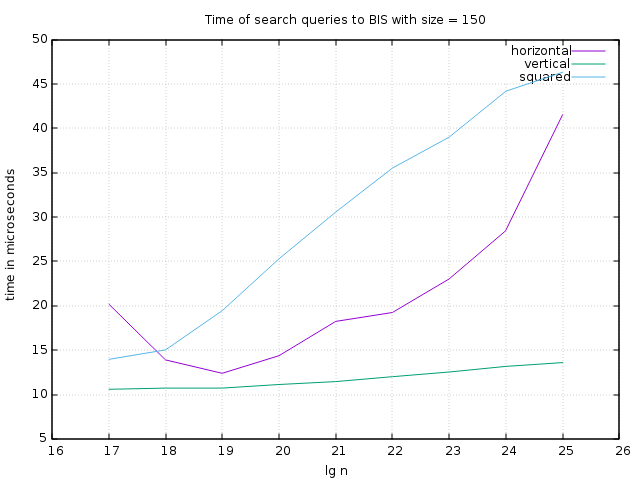
\includegraphics[width=0.99\textwidth]{pictures/analysis/smalls/all_150.png}
        \caption{Queries to the BIS data structure with $size=150$.}
        \label{fig:all_150}
    \end{subfigure}
  }
  \caption{Comparison of shapes on BIS.}
  \label{fig:all_50_and_150}
  
\end{figure}
\clearpage


We look at figure~\ref{fig:all_kdtree_100} in order to confirm that changing the shape from a square to a slice impacts the running time of the search query to kd-tree very much. Comparing figure~\ref{fig:all_100} and figure~\ref{fig:all_kdtree_100} we see that the difference between the two kinds of search queries are much, much bigger on the kd-tree than on the BIS data structure. The biggest ratio between the vertical slice and the square search on figure~\ref{fig:all_100} is around $4$ af $\lg n = 25$. The biggest ratio between he slice and square search on figure~\ref{fig:all_kdtree_100} is around $53$ at $\lg n = 25$. That is really a noticeable difference. Thus, when a search query is performed on the BIS data structure we can expect a much more stable running time. The BIS data structure is more resilient to the shape of the search query than the kd-tree. Figure~\ref{fig:all_50} and figure~\ref{fig:all_150} shows the same tendency as figure~\ref{fig:all_100}: A stable relationship between the square search and slice search with only around a factor $4$ in difference. \\

In section~\ref{sect:squares} we plotted the ratio between a square query to the kd-tree and a square query to the BIS data structure in order to find out how much better the kd-tree performed. Now the roles are reversed, and we are now interested in seeing how much better the BIS data structure performs. 


\begin{figure}[h]
  \makebox[\linewidth][c]{
    \centering
    \begin{subfigure}[b]{0.68\textwidth}
        \centering
        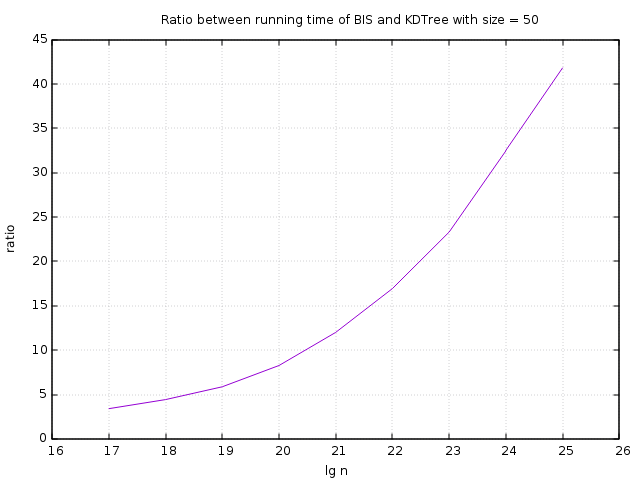
\includegraphics[width=0.99\textwidth]{pictures/analysis/factor_difference_vert_50.png}
        \caption{Ratio with $size=50$.}
        \label{fig:fact_diff_vert_50}
    \end{subfigure}
    %\hfill
    \begin{subfigure}[b]{0.68\textwidth}
        \centering
        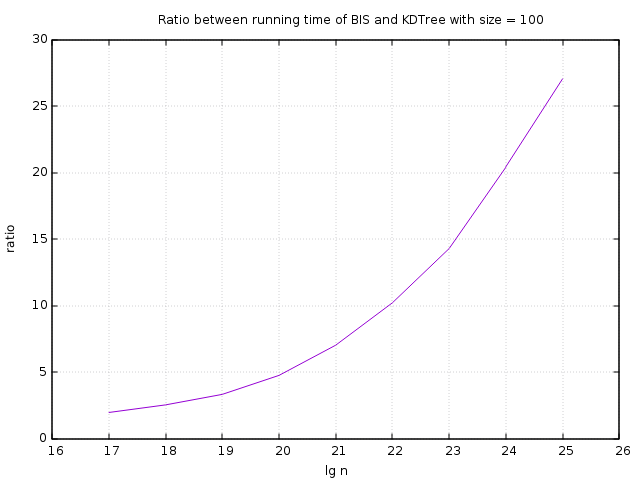
\includegraphics[width=0.99\textwidth]{pictures/analysis/factor_difference_vert_100.png}
        \caption{Ratio with $size=100$.}
        \label{fig:fact_diff_vert_100}
    \end{subfigure}
  }
  \caption{Ratio between BIS data structure and kd-tree with vertical slice. Describes how much better the BIS data structure performs compared to the kd-tree.}
  \label{fig:fact_diff_vert_50_100}
  
\end{figure}


\begin{figure}[h]
    \centering
    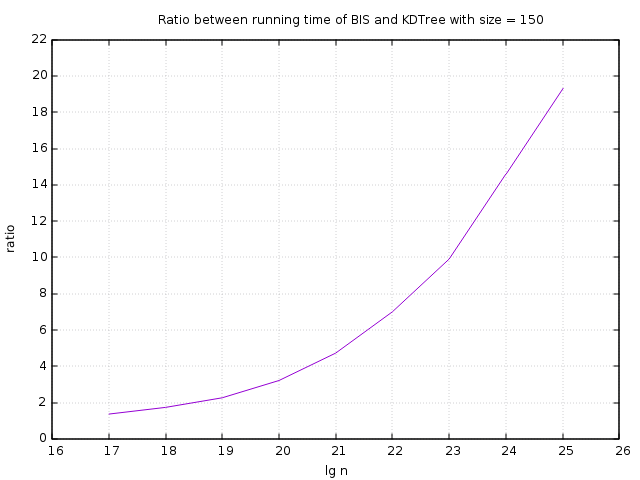
\includegraphics[width = 0.85\textwidth]{pictures/analysis/factor_difference_vert_150.png}
    \caption{Ratio between BIS data structure and kd-tree with $size=150$. Describes how much better the BIS data structure performs compared to the kd-tree.}\label{fig:fact_diff_vert_150}
\end{figure}
\clearpage

\subsection{Worst-case vs best-case}

Figure~\ref{fig:fact_diff_vert_50}, figure~\ref{fig:fact_diff_vert_100} and figure~\ref{fig:fact_diff_vert_150} show the ratio between a vertical slice to the BIS data structure and the kd-tree with a fixed size. Figure~\ref{fig:fact_diff_vert_50} shows that the ratio between grows from $3.5$ to $42$ when $\lg n$ grows from $17$ to $25$. It seems rather reasonable to expect a result size of $50$ from a user interaction. And the more points the data structure holds, the better the ratio between the BIS data structure and the kd-tree. Already at $\lg n = 17$ with a performance increase of a factor of $3.5$ the amount of work saved on a server with many concurrent users is good. Anything above a factor of $10$ seems very, very good. Looking at figure~\ref{fig:fact_diff_vert_100} and figure~\ref{fig:fact_diff_vert_150} we see that the ratio at $\lg n = 25$ has decreased to $27$ and $19$, respectively. They have dropped a lot, but they are still huge factors. With this configuration the BIS data structure is obviously doing a lot better than the kd-tree.




\begin{figure}[h]
  \makebox[\linewidth][c]{
    \centering
    \begin{subfigure}[b]{0.68\textwidth}
        \centering
        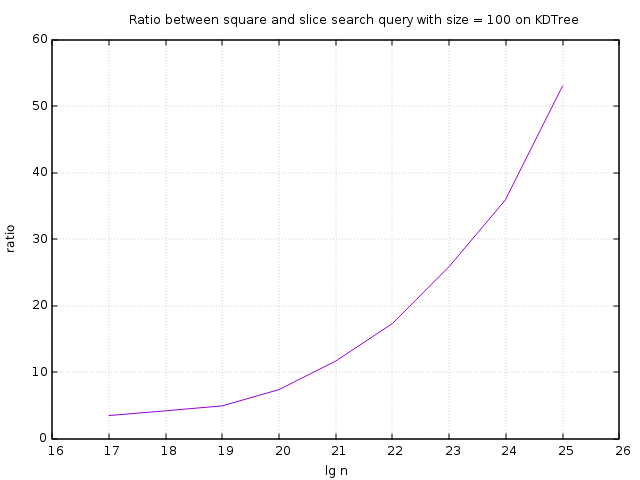
\includegraphics[width=0.99\textwidth]{pictures/analysis/smalls/kdtree_ratio_100.png}
        \caption{Ratio between square and slice search queries to the KDTree with $size=100$.}
        \label{fig:kdtree_ratio_100}
    \end{subfigure}
    %\hfill
    \begin{subfigure}[b]{0.68\textwidth}
        \centering
        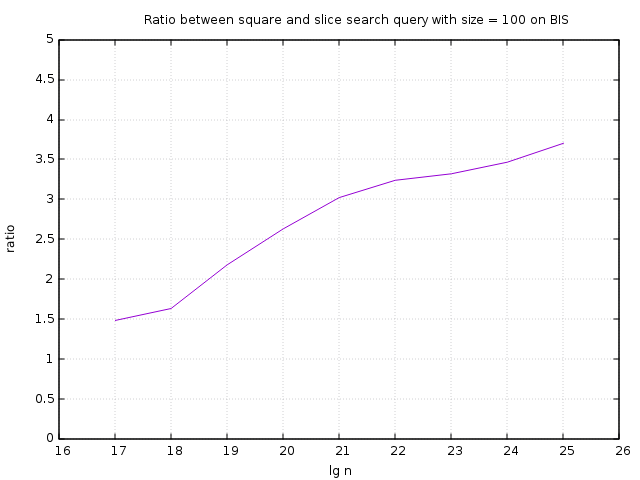
\includegraphics[width=0.99\textwidth]{pictures/analysis/smalls/bis_ratio_100.png}
        \caption{Ratio between square and slice search queries to the BIS with $size=100$.}
        \label{fig:bis_ratio_100}
    \end{subfigure}
  }
  \caption{Comparison of shapes on BIS and KDTree. Ratio describes best-case over worst-case time. KDTree ratio is square over slice and BIS is slice over square. Smaller is better}
  \label{fig:kdtree_bis_ratio_100}
  
\end{figure}

\begin{figure}[h]
  \makebox[\linewidth][c]{
    \centering
    \begin{subfigure}[b]{0.68\textwidth}
        \centering
        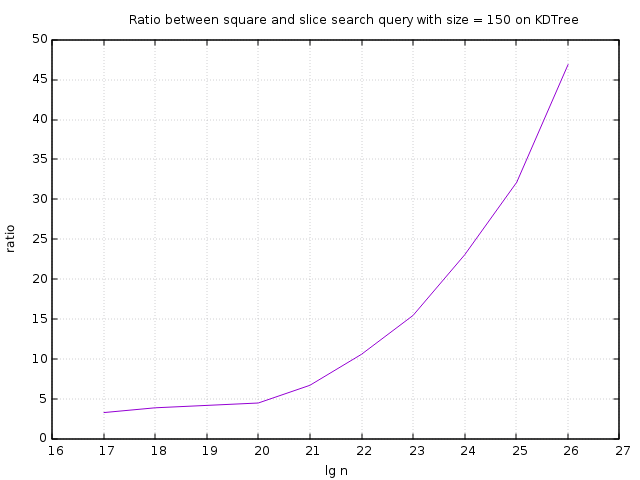
\includegraphics[width=0.99\textwidth]{pictures/analysis/smalls/kdtree_ratio_150.png}
        \caption{Ratio between square and slice search queries to the KDTree with $size = 150$.}
        \label{fig:kdtree_ratio_150}
    \end{subfigure}
    %\hfill
    \begin{subfigure}[b]{0.68\textwidth}
        \centering
        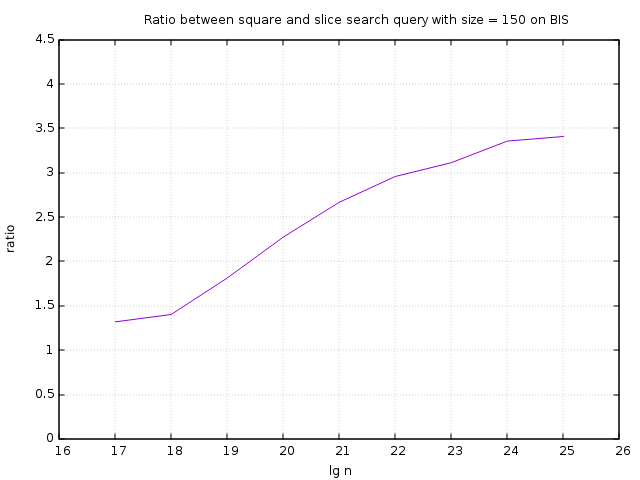
\includegraphics[width=0.99\textwidth]{pictures/analysis/smalls/bis_ratio_150.png}
        \caption{Ratio between square and slice search queries to the BIS with $size = 150$.}
        \label{fig:bis_ratio_150}
    \end{subfigure}
  }
  \caption{Comparison of shapes on BIS and KDTree. Ratio describes worst-case over best-case time. BIS ratio is square over slice and KDTree is slice over square. Smaller is better}
  \label{fig:kdtree_bis_ratio_150}
\end{figure}
  \clearpage

  Figure~\ref{fig:kdtree_ratio_100} shows the ratio between a slice and a square search to the kd-tree. Figure~\ref{fig:bis_ratio_100} shows the ratio between a square and a slice search to the BIS data structure. This ratio describes the worst-case search query divided by the best-case search query. Optimistically we want this ratio to be as close to $1$ as possible. If it is $1$ there is no difference between the square and slice search query, and thus the data structure has a very stable performance. Looking at figure~\ref{fig:kdtree_ratio_100} we see that ratio at $\lg n = 17$ is $3.5$. As $n$ grows, the ratio grows. The ratio at $\lg n = 25$ is $53$. This is not a stable performance between the two shapes of search queries. Figure~\ref{fig:bis_ratio_100} shows that when $\lg n$ grows from $17$ to $25$ the ratio between the square search and the vertical slice search grows from $1.5$ to $3.65$. Thus, the BIS data structure is much more stable in its performance when $k = 100$.

  Figure~\ref{fig:kdtree_ratio_150} and figure~\ref{fig:bis_ratio_150} show the ratio between the two search queries with $size = 150$. Looking at both figures, overall all the ratios have decreased. There is a slight decrease in the ratios on figure~\ref{fig:bis_ratio_150}. The ratio at $\lg n = 17$ is now $1.35$ and the ratio at $\lg n = 25$ is $3.45$. So not a huge drop. This is also a good sign that changing the size of search queries will not impact the ratio too much. Figure~\ref{fig:kdtree_ratio_150} shows that the ratio for the kd-tree has also dropped when the size of the search query has been increased. The ratio at $\lg n = 17$ is now $3.3$ and the ratio at $\lg n = 25$ is $47$. That is still a pretty big difference. And big ratios. It seems that the BIS data structure has a much more stable performance when changing the shape of the search queries.

\todo{Kort opsummering}


  \todo{We use ``size'' and ``k'' interchangably}
  \todo{Fiks captions og titles til de her grafer}
 

\section{Different BIS data structures with $B$ varying}

So far we have only looked at the BIS data structure with $B = \lceil \frac{1}{2}\lg^{\frac{1}{3}} n \rceil$. For $n \in [2^{17}, 2^{25}]$ this is $B=2$. We have also not yet mentioned the important aspect of how much main memory the BIS data structure uses compared to the kd-tree. In this section we are going to look at the BIS data structure for $n \in [2^{17}, 2^{25}]$ and $B={2,3,4}$ and show how much space it uses and compare it to the space used by the kd-tree. We will also look at how well the vertical and horizontal slices perform with $B={3,4}$ by looking at when the query time for a search query to BIS data structure intersects the query time for a search query to the kd-tree. When $B$ grows in the BIS data structure, we expect space to drop, but the query time of a range query to grow.

We are going to briefly look at how the BIS data structure performs with $B=\{3,4\}$. Again, we are going to focus on the vertical slices. We start by introducing figure~\ref{fig:3vert} to see at what size the running time of vertical slices to the BIS data structure with $B=3$ intersects with the running time of the same query to the kd-tree. Recall we have already seen these graphs for $B=2$ on figure~\ref{fig:vert_intersection}.

We are going to introduce the exact same graphs for $B=4$. These are seen on figure~\ref{fig:4vert}.



\begin{figure}[h]
  \makebox[\linewidth][c]{
    \centering
    \begin{subfigure}[b]{0.68\textwidth}
        \centering
        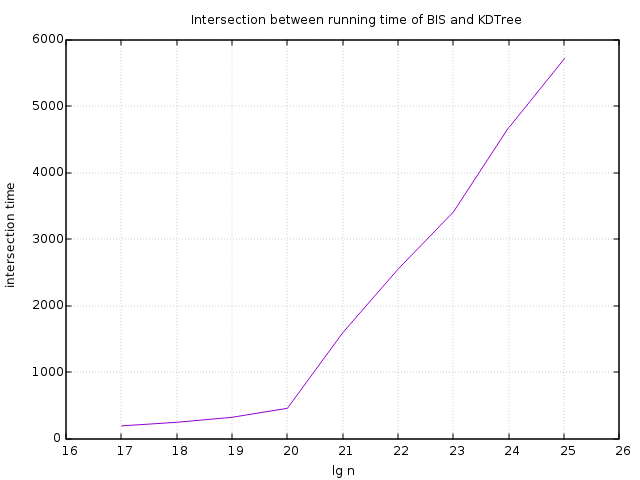
\includegraphics[width=0.99\textwidth]{pictures/analysis/threes/vert.png}
        \caption{Point of intersection with $B=3$.}
        \label{fig:3vert}
    \end{subfigure}
    %\hfill
    \begin{subfigure}[b]{0.68\textwidth}
        \centering
        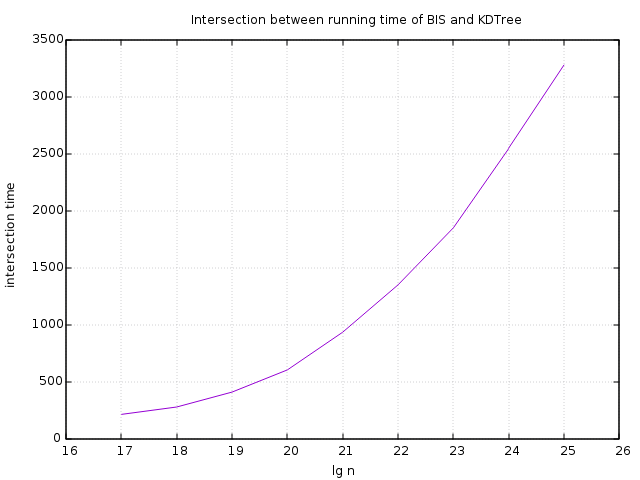
\includegraphics[width=0.99\textwidth]{pictures/analysis/fours/vert.png}
        \caption{Point of intersection with $B=4$.}
        \label{fig:4vert}
    \end{subfigure}
  }
  \caption{Ratio between BIS data structure and kd-tree. Describes how much better the BIS data structure performs compared to the kd-tree.}
  \label{fig:34vert}
  
\end{figure}

\begin{figure}[h]
  \makebox[\linewidth][c]{
    \centering
    \begin{subfigure}[b]{0.68\textwidth}
        \centering
        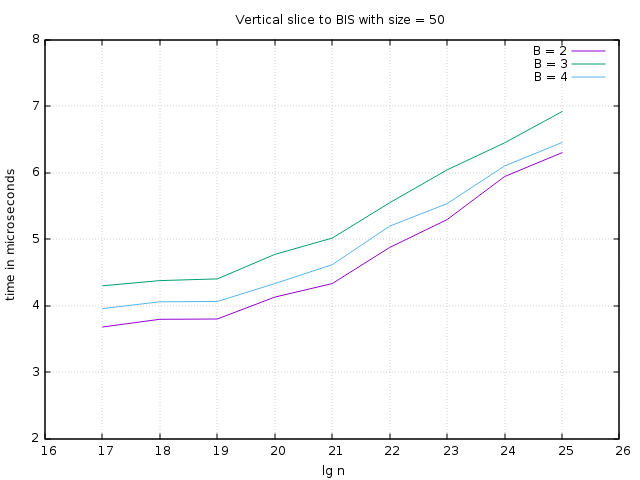
\includegraphics[width=0.99\textwidth]{pictures/analysis/comparing_BIS_50.png}
        \caption{BIS with $size = 50$.}
        \label{fig:BIS_50}
    \end{subfigure}
    %\hfill
    \begin{subfigure}[b]{0.68\textwidth}
        \centering
        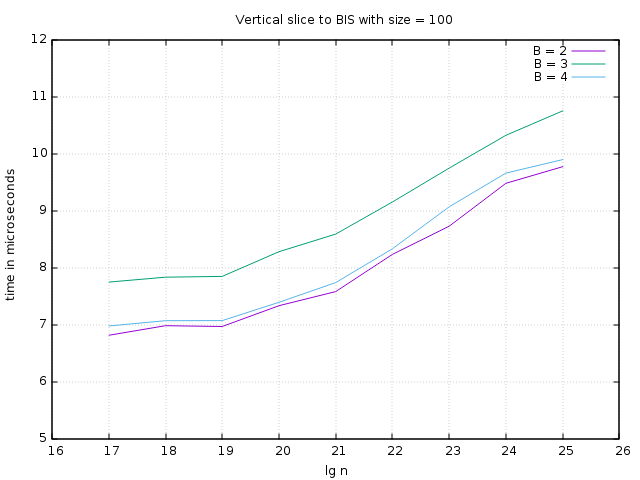
\includegraphics[width=0.99\textwidth]{pictures/analysis/comparing_BIS_100.png}
        \caption{BIS with $size = 100$.}
        \label{fig:BIS_100}
    \end{subfigure}
  }
  \caption{BIS with $B = \{2,3,4\}$. Comparing vertical slices to each}
  \label{fig:comparing_BIS}
  
\end{figure}


The most important reason why the range tree is not used as the standard range reporting data structure today is its space complexity. While we have shown theoretically that the space complexity of the BIS data structure is linear, we would also like to see it in practice. Figure~\ref{fig:sizes} shows the actual space usage of the BIS data structure with $B=\{2,3,4\}$ and the space usage of the kd-tree. The size has been normalized by the amount of points the data structure holds. Thus, the normalized size of the kd-tree is $2$, meaning that for each point in the kd-tree it uses $2\cdot 32$ bits - one $32$ bits integer for each coordinate.

\begin{figure}[h]
    \centering
    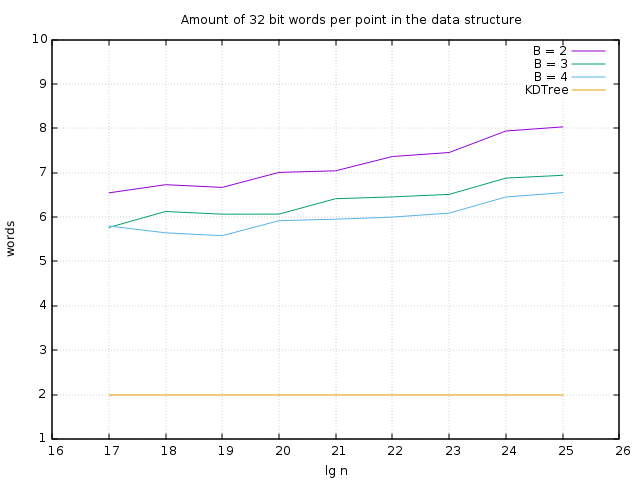
\includegraphics[width = 0.85\textwidth]{pictures/analysis/sizes.png}
    \caption{The normalized sizes of the BIS data structure with $B=\{2,3,4\}$ and the kd-tree.}\label{fig:sizes}
\end{figure}
\clearpage


An interesting thing to remember is that the size of the kd-tree is entirely dependent on the data type used to represent each coordinate. In our experiments we have used a $32$ bit unsigned integer. If we were to change that to a $64$ bit unsigned integer, the size of the kd-tree would increase by a factor of $2$. As the kd-tree, the BIS data structure uses $2$ words per point to store the coordinates. The BIS data structure also uses $1$ word per point to store the y-coordinates in a sorted list as to allow for binary search to find $\hat{y_1}$ and $\hat{y_2}$. The rest of the BIS data structure are no dependent on the data type used to represent the coordinates. Thus, changing the data type from a $32$ bit integer to a $64$ bit integer would only increase the total space usage by $3$ $32$-bit integers per point. On figure~\ref{fig:sizes} the size of the BIS data structure with $B=2$ and $\lg n = 25$ is $8$. Increasing that to $11$ would increase the space usage of the BIS data structure by a factor of $\frac{11}{8} = 1.375$.

The BIS data structure With $B = \lceil \frac{1}{2}\lg^{\frac{1}{3}} n \rceil = 2$ and $\lg n \leq 25$, we get a good performance with certain queries and a better stability when changing the shapes compared to the kd-tree. 


\section{Vertical and horizontal slices explained}
\label{sect:verthoriexp}

In this we are going to dive a deeper into the technical details of the results seen in some of the previous sections. The figures depicting the performance of the vertical slices showed some interesting tendencies. This is the last section before the summary.

\begin{figure}[h]
    \centering
    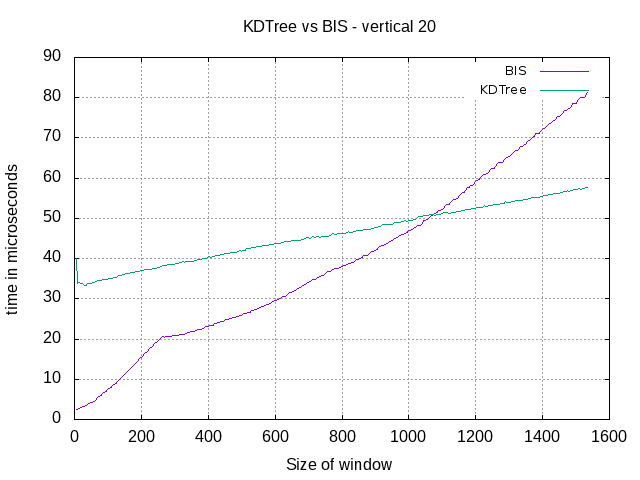
\includegraphics[width = 0.85\textwidth]{pictures/analysis/vert_20.png}
    \caption{Vertical slice. data set size of $n=2^{20}$.}\label{fig:vert_20}
\end{figure}


\begin{figure}[h]
  \makebox[\linewidth][c]{
    \centering
    \begin{subfigure}[b]{0.68\textwidth}
        \centering
        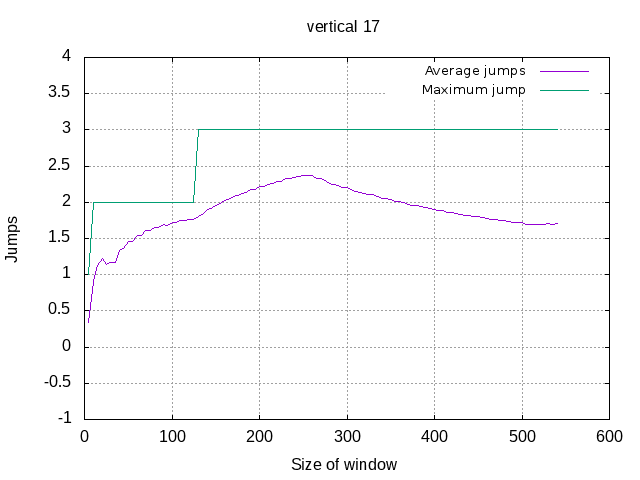
\includegraphics[width=0.99\textwidth]{pictures/analysis/jump_vert_17.png}
        \caption{Data set with $size = 2^{17}$.}
        \label{fig:jump_vert_17}
    \end{subfigure}
    %\hfill
    \begin{subfigure}[b]{0.68\textwidth}
        \centering
        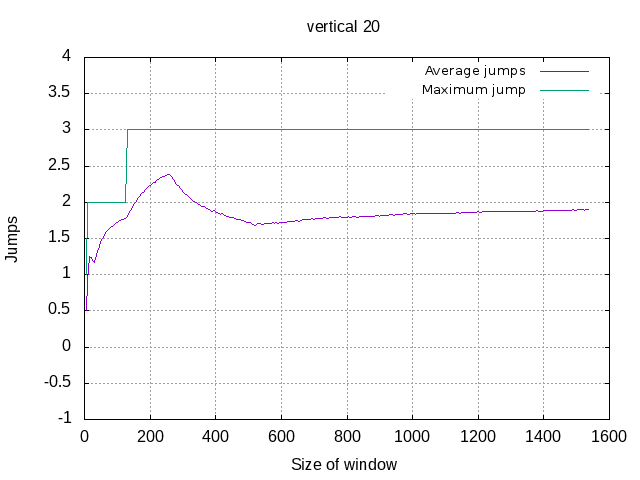
\includegraphics[width=0.99\textwidth]{pictures/analysis/jump_vert_20.png}
        \caption{Data set with $size = 2^{20}$.}
        \label{fig:jump_vert_20}
    \end{subfigure}
  }
  \caption{Size of jumps. 'Average jumps' is the average of all the jumps performed normalized by the size of the slice.}
  \label{fig:jump_vert}
  
\end{figure}



\begin{figure}[h]
  \makebox[\linewidth][c]{
    \centering
    \begin{subfigure}[b]{0.68\textwidth}
        \centering
        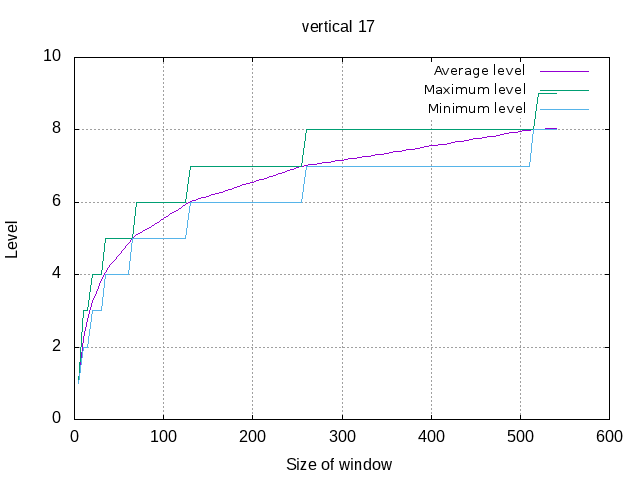
\includegraphics[width=0.99\textwidth]{pictures/analysis/level_vert_17.png}
        \caption{Data set with $size = 2^{17}$.}
        \label{fig:level_vert_17}
    \end{subfigure}
    %\hfill
    \begin{subfigure}[b]{0.68\textwidth}
        \centering
        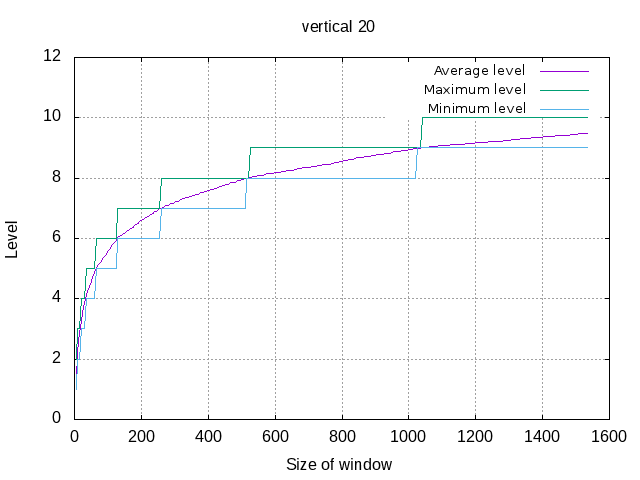
\includegraphics[width=0.99\textwidth]{pictures/analysis/level_vert_20.png}
        \caption{Data set with $size = 2^{20}$.}
        \label{fig:level_vert_20}
    \end{subfigure}
  }
  \caption{Level of highest fully contained node.}
  \label{fig:level_vert}
  
\end{figure}
\clearpage

On the graphs showing the performance of the vertical slices to the BIS data structure, there is a very noticeable change in slope at around $k=256$. Since $B=2$, we have a big jump at level $2^3 = 8$ which allows the ball inheritance structure to jump from level $8$ to a leaf in one jump. When jumping from level $8$ instead of $5$, $6$ or $7$ the ball reaches the leaf in one jump instead of two or three. This means that the average amount of jumps per result will decrease and thus the running time will not increase as fast as before.

Figure~\ref{fig:jump_vert_17} and figure~\ref{fig:jump_vert_20} show the average amount of jumps per result, i.e. the sum of all jumps divided by $k$. We see how the graph has a local maximum at around $k=256$ and then the average amount of jumps per result decreases until $k=512$ where it starts increasing at steady level again. Figure~\ref{fig:level_vert_17} and figure~\ref{fig:level_vert_20} describes the highest level of a fully contained node. We see between $k=256$ and $k=512$ that the maximum is level $8$ and the minimum is level $7$ and that the average level increases meaning more and more fully contained node starts using level $8$. Since we have $B=2$, there is a $2$-jump every $2$ levels, a $4$-jump every $4$ levels, an $8$-jump every $8$ levels and a $16$-jump every $16$ levels. This means that at level $7$ the ball inheritance structure needs $3$ jumps to reach a leaf. This is why such a noticeable local maximum exists on figure~\ref{fig:jump_vert_17} and figure~\ref{fig:jump_vert_20}. The jumps per results eases off because from level $8$ there is $1$ jump, from level $9$ there are $2$ jumps and from level $10$ there are $2$ jumps. The graph on figure~\ref{fig:jump_vert_17} also shows that when $2^i \leq k \leq 2^{i+1}$ the maximum level of the highest fully contained node is $i$ and the minimum level of the highest fully contained node is $i-1$. Recall that the way the vertical slices work means that if a node is fully contained then all of the balls in the node's list will be followed.


%In order to explain this relation between $k$ and the level of the highest fully contained node we look at figure~\ref{fig:level_vert_17}. We see that when we reach $k=256$ the minimum highest level rises to $7$ and the maximum highest level rises to $8$. In order to write the sum of $256<k<512$ we will need to at least level $7$ because we need the two fully contained nodes from level $7$ giving us $2*2^7 = 2^8 = 256$ nodes. If the least common ancestor is found at level $9$ the first fully contained node can be found at level $7$. If all the levels from level $7$ to level $1$ only have fully contained nodes, we get $k = 2*2^1 + 2*2^2 + \cdots + 2*2^7 = 508 < 512$ points. This is not enough to return $512$ points, and thus somewhere between $k=256$ and $k=512$, the search algorithm will begin using level $10$ as the least common ancestor. In a vertical slice, when a node is fully contained, we get all of points in its subtree.


\begin{figure}[h]
    \centering
    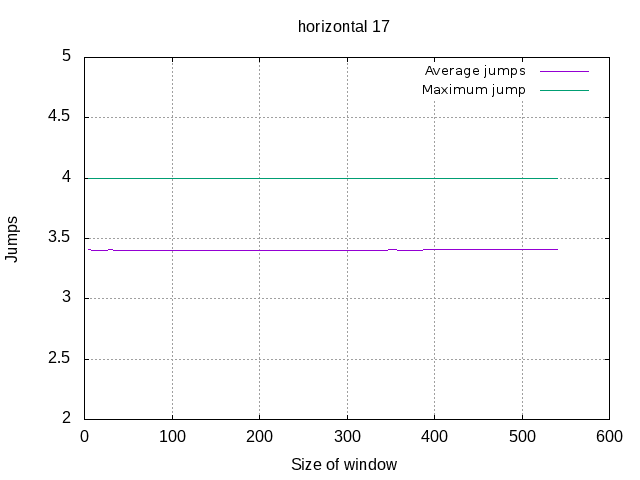
\includegraphics[width = 0.85\textwidth]{pictures/analysis/jump_hori_17.png}
    \caption{Size of jumps - data set size of $n=2^{17}$. 'Average jumps' is the average of all the jumps performed normalized by the size of the slice}\label{fig:jump_hori_17}
\end{figure}
\clearpage

It is a little harder to argue about the horizontal slices. When the least common ancestor of $x_1$ and $x_2$ is found at the root at level $i$, the first node which is fully contained in a horizontal slice is located on level $i-2$. So from level $i-2$ to level $1$ we find $2$ fully contained nodes per level. The points are uniformly distributed which means that given one y-rank of a points, the probability of finding the ball pointing to the leaf of that point on level $i-2$ is $2\cdot\frac{1}{4} = \frac{1}{2}$. The chance to find it on level $i-3$ is half of that, i.e. $\frac{1}{4}$. This trend continues down to level $1$. Thus, we expect the graph of the horizontal slices to be linear because the average amount of jumps should always be same when $n$ is fixed. We can see this on figure~\ref{fig:jump_hori_17}. The figure shows the average amount of jumps divided by the amount of results. The same concept figure~\ref{fig:jump_vert_17} shows. 

This seemingly uninteresting graph shows us that the theory of the expected distribution is correct. We also had this confirmed in section~\ref{sect:squares} where we saw that square searches with the dimensions $[\sqrt{n}\cdot\sqrt{k} \times \sqrt{n}\cdot\sqrt{k}]$ returned $k$ results. This was based on theory that assumed the distribution was uniform. If the y-coordinates are uniformly distributed amongst the x-coordinates to generate a point, we can see something interesting in figure~\ref{fig:jump_hori_17}. A BIS data structure with data set size $n = 2^{17}$ will have its first fully contained node at level $15$. For each y-coordinate we have to find, there is a $\frac{2}{4} = \frac{1}{2}$ chance that it will jump from level $15$. Then there is a $\frac{1}{4}$ chance that it will jump from level $14$ and so on. Given this information we can multiply the probability of using a certain level with the amount of jumps that level uses to get to a leaf. For figure~\ref{fig:jump_hori_17} we start $2$ levels below the least common ancestor. This is level $15$. So the average amount of jumps per result should be $\frac{4}{2} + \frac{3}{4} + \frac{3}{8} + \frac{2}{16} + \frac{3}{32} + \frac{2}{64} + \frac{2}{128} = 3.391$ jumps. Looking at figure~\ref{fig:jump_hori_17} we can confirm this is correct. We omitted the last part of the sum, as $\frac{2}{128}$ is already small enough.

Comparing the internals of the BIS data structure with the kd-tree it is interesting to see that changing the orientation of the slice from vertical to horizontal has such a huge impact on how it is treated. With this information, we can now see why the vertical slice is better than the horizontal. Especially when the size of the slice is big enough for the search to hit the big jump at level $8$.

\section{Summary}

In this chapter we have presented the results of different experiments on the BIS data structure. We have compared it to the kd-tree. We have also confirmed that the theory of the BIS data structure works well in practice.

The BIS data structure performs very well as a slice, most notably as a vertical slice. A square search query does not perform as well as a slice does on the BIS data structure. However the square search query is not a disaster on the BIS data structure. We noticed the difference in performance between the square and slice-formed search query to the BIS data structure was not as big as the difference in performance between the two shapes on the kd-tree. The worst kind of test for the kd-tree was a slice and the best was a square - the exact opposite of the BIS data structure. 

The kd-tree is much more dependent on the shape of its search query than the BIS data structure. This is most notable by looking at the difference between figure~\ref{fig:all_100} and figure~\ref{fig:all_kdtree_100}.



\chapter{Conclusion}
\label{ch:conclusion}


\epigraph{``Hell... It's about time."}{--- \textup{Tychus Findlay}, Starcraft II}

In this thesis we have presented the theory and performance of the BIS data structure. We have compared the performance of the BIS data structure to that of the kd-tree. The performance of the BIS data structure corresponds well with the theoretical running time of $\mathcal{O}(\lg n + k\cdot\lg^\epsilon n)$. It does not seem like the theoretical query time has any hidden big constants like we assumed the OBIS data structure had.

We have seen that, just like the kd-tree, the BIS data structure has a worst-case search query and a best-case search query. The difference in execution time between the worst-case and best-case search query to the BIS data structure is much less than that of the kd-tree. We have seen that the search query to the BIS data structure performs much more stable than a search query to the kd-tree.

Given a search query in the shape of slice, the BIS data structure will outperform the kd-tree up to good size. With $2^{17}$ points and a vertical search query, the BIS data structure will outperform the kd-tree when $k$ is less than $200$. With $2^{25}$ points and a vertical search query, the BIS data structure will outperform the kd-tree when $k$ is less than $4660$. 

For smaller sizes of $k$, a vertical query to the BIS data structure will be several times faster than the kd-tree. With $2^{17}$ points and a vertical search query, the BIS data structure will be $3.5$ times faster than the kd-tree when $k = 50$. With $2^{25}$ points the BIS data structure will be $42$ times faster than the kd-tree when $k = 50$. In general the BIS data structure performs pretty well for when $k$ is small. It can definitely compete with the kd-tree.

There is a duality between the shapes of the search queries to the BIS data structure and the kd-tree. The BIS data structure performs best with slices and the kd-tree performs best with square searches. The BIS data structure performs worst with the square search and the kd-tree performs worst with a slice.

We have seen that the BIS data structure actually does compete with the kd-tree. The BIS data structure could be a realistic alternative to the kd-tree in practice. By picking an $\epsilon$ and a $c$ for $B = c\cdot\lg^\epsilon n$ we are able to leverage the performance of the BIS data structure with the amount of main memory it should be able to use.


%%%%%%%%%%%%%%%%%%%%%%%%%%%%%%%%%%%%%%%%%%%%%%%%%%%%%%%%%%%%%%%%%%%%%%%

\addcontentsline{toc}{chapter}{Primary Bibliography}
\bibliographystyle{plainnat} 
\bibliography{refs}

\end{document}

